\documentclass{UoNMCHA}
\usepackage[authoryear]{natbib}
\usepackage{array,booktabs} % For nice tables
\usepackage{amsmath,amsfonts,amssymb} % For nice maths
\newcommand{\norm}[1]{\left\lVert#1\right\rVert}
\usepackage{color}
\usepackage{enumerate}
\usepackage{listings}
\usepackage[export]{adjustbox}
\usepackage{subfig}
\usepackage{hyperref}
\usepackage[nameinlink,noabbrev]{cleveref}
\usepackage{pdfpages}
\usepackage{rotating}
\usepackage[parfill]{parskip}   % For replacing paragraph indenting with a newline instead
% Number equations per section
\numberwithin{equation}{section}

\hypersetup{
%    bookmarks=true,         % show bookmarks bar?
%    unicode=false,          % non-Latin characters in AcrobatÕs bookmarks
%    pdftoolbar=true,        % show AcrobatÕs toolbar?
%    pdfmenubar=true,        % show AcrobatÕs menu?
%    pdffitwindow=false,     % window fit to page when opened
%    pdfstartview={FitH},    % fits the width of the page to the window
%    pdftitle={My title},    % title
%    pdfauthor={Author},     % author
%    pdfsubject={Subject},   % subject of the document
%    pdfcreator={Creator},   % creator of the document
%    pdfproducer={Producer}, % producer of the document
%    pdfkeywords={keyword1} {key2} {key3}, % list of keywords
%    pdfnewwindow=true,      % links in new window
    colorlinks=true,       % false: boxed links; true: colored links
    linkcolor=blue,          % color of internal links
    citecolor=blue,        % color of links to bibliography
%    filecolor=magenta,      % color of file links
    urlcolor=blue           % color of external links
}

\definecolor{MATLABKeyword}{rgb}{0,0,1}
\definecolor{MATLABComment}{rgb}{0.1328125,0.54296875,0.1328125}
\definecolor{MATLABString}{rgb}{0.625,0.125,0.9375}

\lstset{language=Matlab,
    basicstyle=\small\ttfamily,
    keywordstyle=\color{MATLABKeyword},
    %identifierstyle=,
    commentstyle=\color{MATLABComment},
    stringstyle=\color{MATLABString},
    numberstyle=\tiny,
    %numbers=left,
    basewidth=0.5em}

\firstpage{1}    % Set page number for first page
\UoNMCHAreportNo{MECH4841 Part B} %Report number
\UoNMCHAyear{2013}   % Year
\shorttitle{FYP Report - Optical Flow Based Obstacle Avoidance} %For odd pages
%%%%%%%%%%%%%%%%%%%%%%%%%%%%%%%
\begin{document}

\includepdf[pages=-]{FYP_Cover_Page.pdf}
\title{Optical Flow Based Obstacle Avoidance for a Fixed Wing UAV\\ \ \\
{\small Final Year Project Report - MECH4841 Part B  \\June 2019}}
\author[UoNMCHA]{Patrick Prell}
\address[UoNMCHA]{
Student of Mechatronics Engineering,\\
The University of Newcastle, Callaghan, NSW 2308, AUSTRALIA \\
Student Number: 3204734 \\
E-mail: \href{mailto:Patrick.Prell@uon.edu.au}{\textsf{Patrick.Prell@uon.edu.au}}}
%%%%%%%%%%%%%%%%%%%%%%%%%%%%%%%
\maketitle
\onecolumn

\vspace{-5mm}
\section*{Abstract}
\vspace{-3mm}
Remember that executive summary may include the following information:
\begin{itemize}
    \item Defines the intention of the report.
    \item Places the report in context so the reader knows why it is important to read it.
    \item Why is it important?
    \item What problem is addressed?
    \item Briefly states the results
    \item Briefly presents the implications and recommendations
\end{itemize}
%%%%%%%%%%%%%%%%%%%%%%%%%%%%%%%
\vspace{-2mm}
\section*{Acknowledgements}
\vspace{-3mm}
You may like to say thank you to someone that helped you with your project.
%%%%%%%%%%%%%%%%%%%%%%%%%%%%%%%
\newpage
\tableofcontents
%%%%%%%%%%%%%%%%%%%%%%%%%%%%%%%
\newpage
\section{Introduction}

Exploring and navagating unknown environments is an essential instinct in biology and avoiding obstacles is an major component. For robotic vehicles to perform high level tasks, they must also have these instincts.

\begin{itemize}
    \item \textbf{Position}: Show there is a problem and that it is important to solve it.
    \item \textbf{Problem}: Describe the specifics of the problem you are trying to address
    \item \textbf{Proposal}: Discuss how you are going to address this problem. Use the literature to back-up your approach to the problem, or to highlight that what you are doing has not been done before
\end{itemize}

The rest of the report is organised as follows. \Cref{sec:Background} describes items related to the core content. \Cref{sec:Conclusion} concludes the report. Appendix~ shows an example of how to make a Table.

% %%%%%%%%%%%%%%%%%%%%%%%%%%%%%%%
\newpage
\section{Background}\label{sec:Background} %Checked with grammarly
To the average human or most mammals for that matter, visual tasks such as identifying objects and interpreting visual cues might seem like a trivial task. However, implementing algorithms that mimic a mammalian visual cortex is infuriatingly difficult and largely remains an unsolved problem \citep{hartley2003multiple}. One fact often overlooked is that for all of its amazing abilities, approximately 1/3 of the human brain is dedicated to analysing information collected from our eyes. This statistic helps to put into perspective how challenging the field of computer vision can be.

The concept of computer vision has been explored since the inception of artificial intelligence in the late 1960s. Computer vision was made possible by leaps in computer power, allowing manipulation of large (for the time) data sets such as images and videos. The following decade saw research attempting to extract information from a sequence of images using visual cues embedded in the motion of an image. This brought about research on visual navigation as a viable method for a mobile robot to navigate an environment. Using Visual Navigation on a robot to move through an unstructured environment with no prior knowledge of the map is often based on optical flow. A motion field is estimated from fusing the motion of the robot with the motion of the pixels of a video feed. Furthermore, visual navigation techniques have been inspired by biology. Observing the way that animals and insects utilise their visual systems to move about and map their environments, the processes for which this is achieved can be replicated and implemented on a robotic system \citep{altshuler2018comparison}.

The following section builds the background knowledge required to utilise visual cues as input to an obstacle avoidance system. In particular, a history of visual navigation is outlined;  the geometry of a camera and the tools for calibrating it are introduced; and the kinematics of vision optical flow and optical flow on the view sphere. Finally, this section discusses the approach taken to validate the obstacle avoidance algorithm.

% \subsection{Inverse Optimal Control} % 3 pages

\subsection{Biomimicry} % 1 page %Checked with grammarly
Biology so often holds a wealth of inspiration for engineers. From the material science of the microstructures in a butterfly wing to the computational fluid dynamics of a Kingfisher diving into water \citep{benyus1997biomimicry}. visual sensors are found so frequently in nature, making it very productive to look at nature and tap into the eons of knowledge distilled by evolution.

\subsubsection{Inverse Optimal Control}
The traditional way of designing an autonomous system is to create a cost function for the system and use this cost function to produce an optimal policy. This method often involves tweaking tuning prametrs and weight values that are too complicated to understnd intuitively. This is known as optimal control. as the name suggests, inverse optimal control flips these techniques around. Inverse optimal control can be a far more intuitive method of obtaining the desired behavior from a robot.

Rather than defining a cost function that generates the policy for the robot, inverse optimal control uncovers the cost function that best explains demonstrated optimal behavior \citep{ratliffinverse}. This behavior can be obtained through the intuition of the mechatronics engineer designing the robot. Or this behavior can be derived from biology, such as the work by 
\subsubsection{Visual Navigation}

\subsection{Optical Flow}
In computer vison we are constanly running into the problem of dimentional compression. A lot of information is lost in the projection from 3 dimentions to a 2D plane, and when that projection is inverted, the lost data needs to be inferred. In the case of optical flow, the lost data comes mainly from different assumptions that are made to make the optic flow algorithm solvable. Each Optical flow algorithm has its own set of assumptions and constraints.

Beginnning with a basic description of optical flow. Optic flow is the apparent movement of objects, textures and edges between a sequence of frames. Optic flow can be thought of as the time derivitive of two images. It is dificult to imagine daking the derivitive of an image, and it is this which makes evaluating optic flow so dificult. One major probem with calculating optic flow is the \textit{aperture problem}. This probelm manifests in many optical illutions that trick the human brain aswell. An example of this effect can be seen in \ref{fig:ApertureProblem}. To an unassuming camera, it is impossible to tell the direction of the striped pattern.

\begin{figure}[ht]
    \begin{center}
        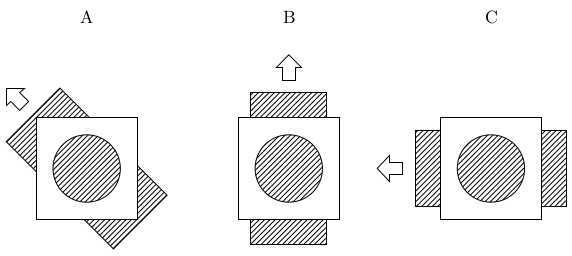
\includegraphics[width=.6\linewidth]{Figures/ApertureProblem}
        \caption{The direction of the stripes through the aperture is unclear without more context}
        \label{fig:ApertureProblem}
    \end{center}
\end{figure}


There have been many solutions proposed to calculate the motion of pixels in an image. Each method being designed for different tasks and having their own set of advantages and disadvantags for their particular situation. The following section outlines two  early methods for calculating optical flow, these being the \textit{Horn and Schunk} and \textit{Lucas - Kanade} method. Although both of these methods were devised over 20 years ago, they have layed a foundation for many optic flow algorithms following \citep{sun2010secrets}. The farnback algorithm, a much more recent algoithm will then be discussed as this is the algorithm used for the project.

\subsubsection{Horn \& Schunk}
Horn and Schunck optic flow is based around an assumption known as the \textit{Brightness constancy}. This says that the intencity of a pixel remains constant over a small step in time.
\begin{equation}
	\frac{dI}{dt} = 0
\end{equation}
Defining a vector field $h = (u, v) = \left(\frac{du}{dt}, \frac{dv}{dt}\right)$ that hold the brightness constancy true, the chain rule is used to derive the following \textit{optic flow constraint} equation.

\begin{equation}
	\nabla I \mathbf{h} + I_{t} = 0
\end{equation}

This equation exposes the aperture problem in \ref{fig:ApertureProblem} mathmatically. There are more variables to solve for than there are linearly independent equations meaning there is no unique solutioin for these variables. in \cite{horn1981determining}, This problem addressed by formulating the estimation of optical flow as a minimisation problem. where the vector field $(u, v)$ is presented as the minimiser for an energy function $J(u, v)$. this energy function is made up of the optic flow constraint based on brightness constancy, and another term based on the gradient of the flow. The following energy function is as follows:
\begin{equation}
	J(u, v) = \int_{\Omega}(I_{x}u + I_{y}v + I_{t})^{2} + \alpha^2(|\nabla u|^{2} + |\nabla v|^{2})
\end{equation}
where $\alpha$ is the weight of the smoothness of the resulting flow field.

Horn and Schunck's optical flow algorithm was a huge step forward in computer vision research, although this algorithm is limited in that it typically can only estimate small motions, the method fails in the presence of large motion when the gradient of the image is not smooth enough \citep{meinhardt2013horn}.

\subsubsection{Lucas - Kanade}
The Lucas-Kanade method is a widely used method for calculating optical flow. This method operates under the assumption that the flow is effectively constant in a small cluster of pixels, the method can then solve the optical flow equation for all the pixels in that neighbourhood using least squares regression. The Lucas-Kanade method improves on previous methods by using the spatial intensity gradient to find the disparity vector $h$, reducing the algorithms calculation time to $O(M^2log(N))$ for the average case.

\subsubsection{What is Observable in Optical Flow}
Pose rate estimation

\begin{itemize}
	\item Angular velocity,
	\item reflect on the work presented, 
	\item make recommendations,
	\item suggest future work or improvements.
\end{itemize}
\subsection{Reference Frames and Coordinate Systems}
In general, the motion of an object needs to be described relative to some coordinate system and the reference frame. Defined by \cite{3900Notes}, a reference frame is a perspective from which the motion is described by an observer. A reference frame can be defined by a set of at least 3 non-colinear points that are rigidly connected. The reference frames used in this project are $\mathcal{C}$, $\mathcal{B}$ and $\mathcal{N}$ for the camera, the vehicle (body) and the world frames respectively.

Furthermore, a coordinate system is a way to describe the position and motion of objects relative to its reference frame. A coordinate system in three-dimensional Euclidean geometry is made up of at least three orthogonal basis vectors of unit length. This report uses the same notation as used in \cite{3900Notes} to describe a vector from point $O$ to point $P$ as $\vec{r}_{P/O}$. \Cref{fig:ReferenceFrame} shows an example reference frame $\mathcal{C}$ attached to a camera with an associated coordinate system $\{c\}$.

\begin{figure}[ht]
    \begin{center}
        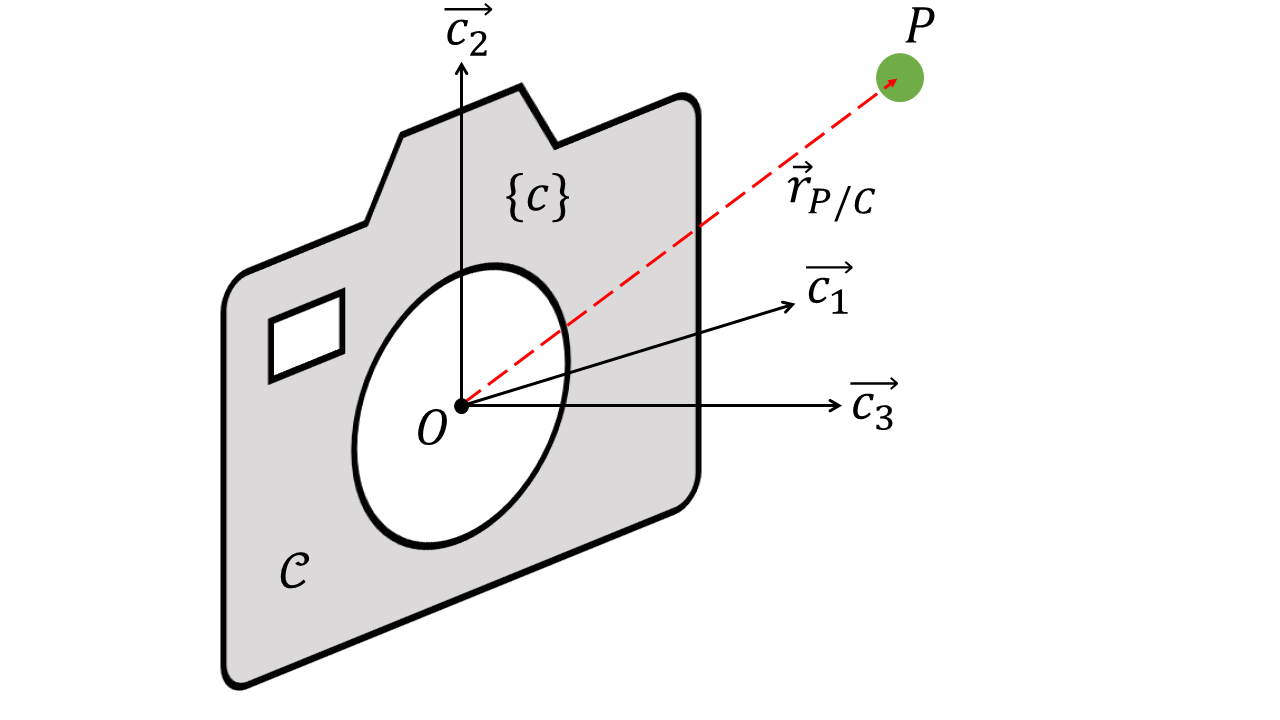
\includegraphics[width=.6\linewidth]{Figures/ReferenceFrame}
        \caption{A reference frame $\mathcal{C}$ with its associated coordinate system $\{c\}$}
        \label{fig:ReferenceFrame}
    \end{center}
\end{figure}

When designing computational models, it is often convenient to represent vectors as column matrices in $\mathbb{R}^3$. The basis of the original vector is denoted as a superscript of the matrix. That is, a vector $\vec{v}$ in basis $\{a\}$ is written as $\mathbf{v}^a$, or more generally: 
\begin{equation}
	\mathbf{v}^a = 
	\begin{bmatrix}
		v^{a}_1\\
		v^{a}_2\\
		v^{a}_3
	\end{bmatrix}
\end{equation}

In this form, the dot product of two vectors $\vec{u} \cdot \vec{v}$ (inner product) in the same basis becomes a matrix operation:
\begin{equation}
	(\mathbf{u}^{a})^{T}\mathbf{v}^{a} = 
	\begin{bmatrix}
		u^{a}_1 & u^{a}_2 & u^{a}_3
	\end{bmatrix}
	\begin{bmatrix}
		v^{a}_1\\
		v^{a}_2\\
		v^{a}_3
	\end{bmatrix}
\end{equation}

Additionally, the cross product of two vectors $\vec{w} = \vec{u}\times\vec{v}$ can be represented as the \textit{skew-symmetric} matrix of $\mathbf{u}^{a}$ multiplied by $\mathbf{v}^{a}$. That is:
\begin{equation}
	\mathbf{w}^{a} = \mathbf{S}(\mathbf{u}^a)\mathbf{v}^a
\end{equation}
The skew-symmetric operator $\mathbf{S(u)}$ arranges the elements in $u$ such that the resulting matrix is skew-symmetric.

\begin{equation}\label{eq:SkewSymmetric}
	\mathbf{S}(\mathbf{u}) = 
	\begin{bmatrix}
		0 & -u_{3} & u_{2}\\
		u_{3} & 0 & -u_{1}\\
		-u_{2} & u_{1} & 0
	\end{bmatrix}
\end{equation}

\subsubsection{Coordinate Transforms and Rotation Matrices}
This project uses multiple coordinate systems to deal with the complex geometry of the camera and vehicle. Therefore, in order to have context for measurements and actions of different sensors and actuators, their orientation needs to be transformed into the relevant coordinate system. The following report will use rotation matrices, as derived from a coordinate transform.

A vector can be described from multiple bases, for instance, $\vec{r}$ can be represented in both basis $\{n\}$ and basis $\{c\}$ as:
\begin{equation}\label{eq:uInAandB}
	\begin{split}
		\vec{r} &= r^{n}_{1}\vec{n}_{1} + r^{n}_{2}\vec{n}_{2} + r^{n}_{3}\vec{n}_{3}\\
		\vec{r} &= r^{c}_{1}\vec{c}_{1} + r^{c}_{2}\vec{c}_{2} + r^{c}_{3}\vec{c}_{3}
	\end{split}
\end{equation}

Expressing $\vec{r}$ as an inner product of the basis $\{c\}$ and $r^{n}$:
\begin{equation}
	\vec{r} = 
	\begin{bmatrix}
		\vec{c}_{1} & \vec{c}_{2} & \vec{c}_{3}
	\end{bmatrix}
	\begin{bmatrix}
		r^{c}_{1}\\
		r^{c}_{2}\\
		r^{c}_{3}
	\end{bmatrix}
\end{equation}
Finally, express both sides in $\{n\}$:
\begin{equation}
	\mathbf{r}^{n} =
	\begin{bmatrix}
        \mathbf{b}^{c}_{1} & \mathbf{b}^{c}_{2} & \mathbf{b}^{c}_{3}
	\end{bmatrix}
	\mathbf{u}^{c}
\end{equation}
This can be denoted more generally in matrix form:
\begin{equation}
	\mathbf{r}^{c} = \mathbf{R}^{c}_{n}\mathbf{r}^{n}.
\end{equation}

In robotics, it is often desirable to rotate a vector to a particular angle. The method used in this project is known as \textit{euler rotation}. Euler angles discretise a complex three-dimensional rotation into three separate planar rotations about each basis vector. The rotation matrices about each basis vector are given by:
\begin{equation}\label{eq:planarRotations}
	\begin{split}
		\mathbf{R}_{x}(\phi) &= 
		\begin{bmatrix}
			1 & 0 & 0\\
			0 & cos(\phi) & -sin(\phi) \\
			0 & sin(\phi) & cos(\phi)
		\end{bmatrix}\\
		\mathbf{R}_{y}(\theta) &= 
		\begin{bmatrix}
			cos(\theta) & 0 & sin(\theta)\\
			0 & 1 & 0 \\
			-sin(\theta) & 0 & cos(\theta)
		\end{bmatrix}\\
		\mathbf{R}_{z}(\psi) &= 
		\begin{bmatrix}
			cos(\psi) & -sin(\psi) & 0\\
			sin(\psi) & cos(\psi) & 0 \\
			0 & 0 & 1
		\end{bmatrix}
	\end{split}
\end{equation}

The order of these rotations effects the final position, for this reason in this project the common robotics convention of \textit{Roll, Pitch, Yaw} (RPY) will be used. The notation for a rotation matrix from $\{n\}$ to $\{c\}$ is given by $\mathbf{\Theta}^{n}_{c}  \triangleq \begin{bmatrix}\phi & \theta & \psi\end{bmatrix}^\top$. using the consecutive planar rotations from \cref{eq:planarRotations} we get $r^{b}_{a} = \mathbf{R}_{z}(\psi)\mathbf{R}_{y}(\theta)\mathbf{R}_{x}(\phi)r^{a}_{b} = \mathbf{R}(\mathbf{\Theta}^{n}_{c})r^{a}_{b}$. From this, the structure of a full rotation matrix:
\begin{equation}
	\mathbf{R}(\mathbf{\Theta}^{n}_{c}) = 
	\begin{bmatrix}
		c_{\psi} c_{\theta} & −s_{\psi} c_{\phi} + c_{\psi} s_{\theta} s_{\phi} & s_{\psi} s_{\phi} + c_{\psi} c_{\phi} s_{\theta}\\
		s_{\psi} c_{\theta} & c_{\psi} c_{\phi} + s_{\phi} s_{\theta} s_{\psi} &  −c_{\psi} s_{\phi} + s_{\psi} c_{\phi} s_{\theta}\\
		−s_{\theta} & c_{\theta} s_{\phi} & c_{\theta} c_{\phi}		
	\end{bmatrix}
\end{equation}
where $s  \triangleq sin(\mathbf{\cdot})$ and $c  \triangleq cos(\mathbf{\cdot})$.

Due to the orthogonality of rotation matrices, they have the property that the inverse of the rotation matrix is equal to its transpose:
\begin{equation}
	\mathbf{R}^{-1} = \mathbf{R}
\end{equation}
This is useful, as rotating a vector back to its original orientation is as simple as applying the transposed rotation matrix. That is $\mathbf{R}^{b}_{a} = \mathbf{R}^{a\top}_{b}$.
\subsection{Kinematics of Vision}
While discussing the motion of objects in a space, it is helpful to properly define a geometric definition for these points and the relative motion between them. Kinematics defines these such relationships. More specifically, kinematics defines the reference frame from which the motion of a point can be described and the transformation that associates this motion in a separate reference frame. These concepts will be used to describe the relative motion between a camera mounted on a vehicle in an environment.

\subsubsection{Time Derivative of Vectors and Transport Theorem}\label{sec:VectorDerivitives}
The subtle difference between the time-derivative of a scalar magnitude and a vector magnitude is that the vector derivative depends on the reference frame from which they are being observed \cite{3900Notes}. \Cref{fig:vectorDerivitive} shows a vector $\vec{r}$ observed from two separate reference frames, $\mathcal{A}$ and $\mathcal{B}$.

\begin{figure}[ht]
    \begin{center}
        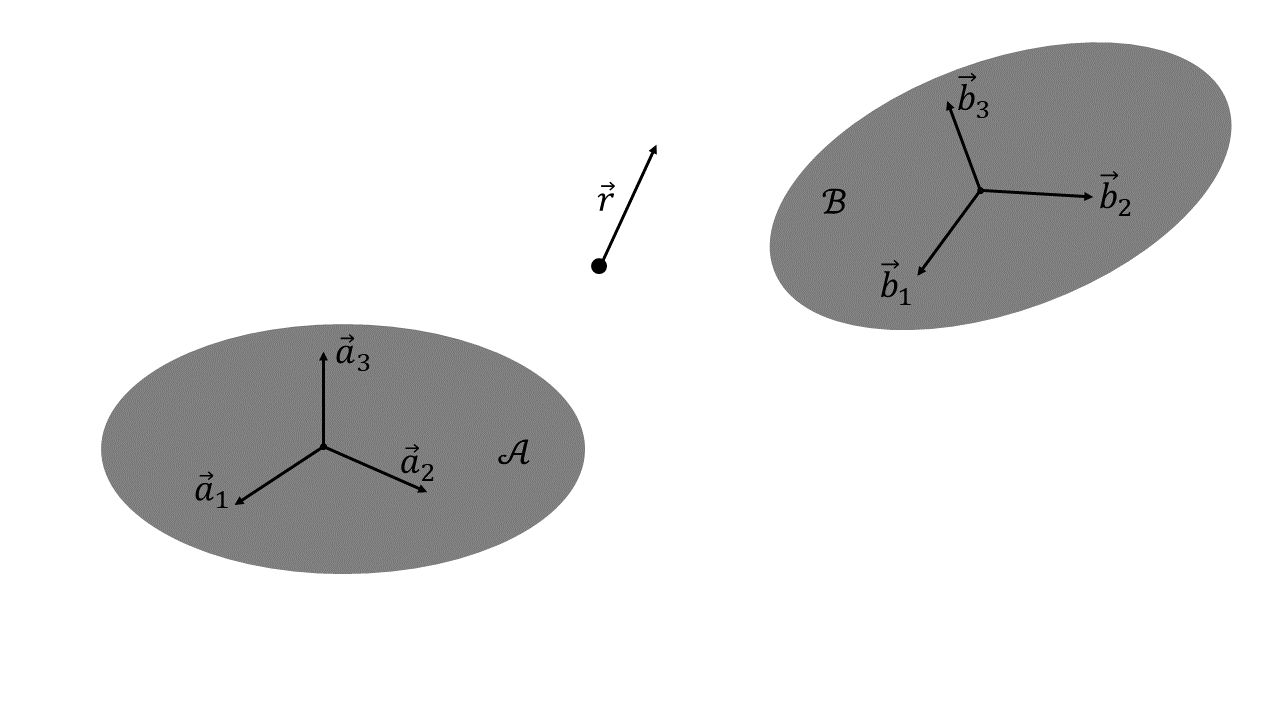
\includegraphics[width=.8\linewidth]{Figures/vectorDerivitive}
        \caption{A vector $\vec{r}$ seen from two reference frames.}
        \label{fig:vectorDerivitive}
    \end{center}
\end{figure}

Taking the time derivative of $\vec{r}$ in each vector frame:

\begin{equation}
	\begin{split}
		\frac{{}^\mathcal{A}d\vec{r}}{dt} &= \frac{dr^{a}_{1}}{dt}\vec{a}_{1} + \frac{dr^{a}_{2}}{dt}\vec{a}_{2} + \frac{dr^{a}_{3}}{dt}\vec{a}_{3}\\
		\frac{{}^\mathcal{B}d\vec{r}}{dt} &= \frac{dr^{b}_{1}}{dt}\vec{b}_{1} + \frac{dr^{b}_{2}}{dt}\vec{b}_{2} + \frac{dr^{b}_{3}}{dt}\vec{b}_{3}\\
	\end{split}
\end{equation}
Consider the case of a frisbee flying through the air carrying a spider $S$ as a passenger. Reference frame $\mathcal{F}$ is attached rigidly to the frisbee and an observer $O$ is watching it from the field in reference frame $\mathcal{O}$. Clearly, the movement of the spider is different from $\mathcal{A}$ as it is from $\mathcal{F}$ or more generally:
\begin{equation}
		\frac{{}^\mathcal{O}d\vec{r}}{dt} \neq \frac{{}^\mathcal{F}d\vec{r}}{dt}
\end{equation}
To find the time derivative of the spider relative to $\mathcal{O}$, two methods could be used: the time derivative of the vector $\vec{r}_{S/O}$ can be taken, which will prove to be a tedious exercise. Or the \textit{transport theorem} can be used.

In accordance with \cite{3900Notes}, the transport theorem states that there exists a unique vector $\vec{\omega}_{\mathcal{B}/\mathcal{A}}$ called the \textbf{angular velocity} of $\mathbf{\mathcal{B}}$ with respect to $\mathbf{\mathcal{A}}$ such that:
\begin{equation}\label{eq:transportTheorem}
	\frac{{}^\mathcal{A}d\vec{r}}{dt} = \frac{{}^\mathcal{B}d\vec{r}}{dt} + \vec{\omega}_{\mathcal{B}/\mathcal{A}}\times\vec{r}
\end{equation}
Using the transport theorem, the velocity of the spider relative to $\mathcal{O}$ is simply the velocity of the frisbee's centre $P$ plus the rotational velocity of the frisbee, resulting in:
\begin{equation}
	\frac{{}^\mathcal{O}d}{dt}\vec{r}_{S/O} = \frac{{}^\mathcal{F}d}{dt}\vec{r}_{P/O} + \vec{\omega}_{\mathcal{F}/\mathcal{O}}\times\vec{r}_{P/O}
\end{equation}
\subsubsection{Spherical Flow Model}\label{sec:SphericalFlow}
\begin{figure}[ht]
    \begin{center}
        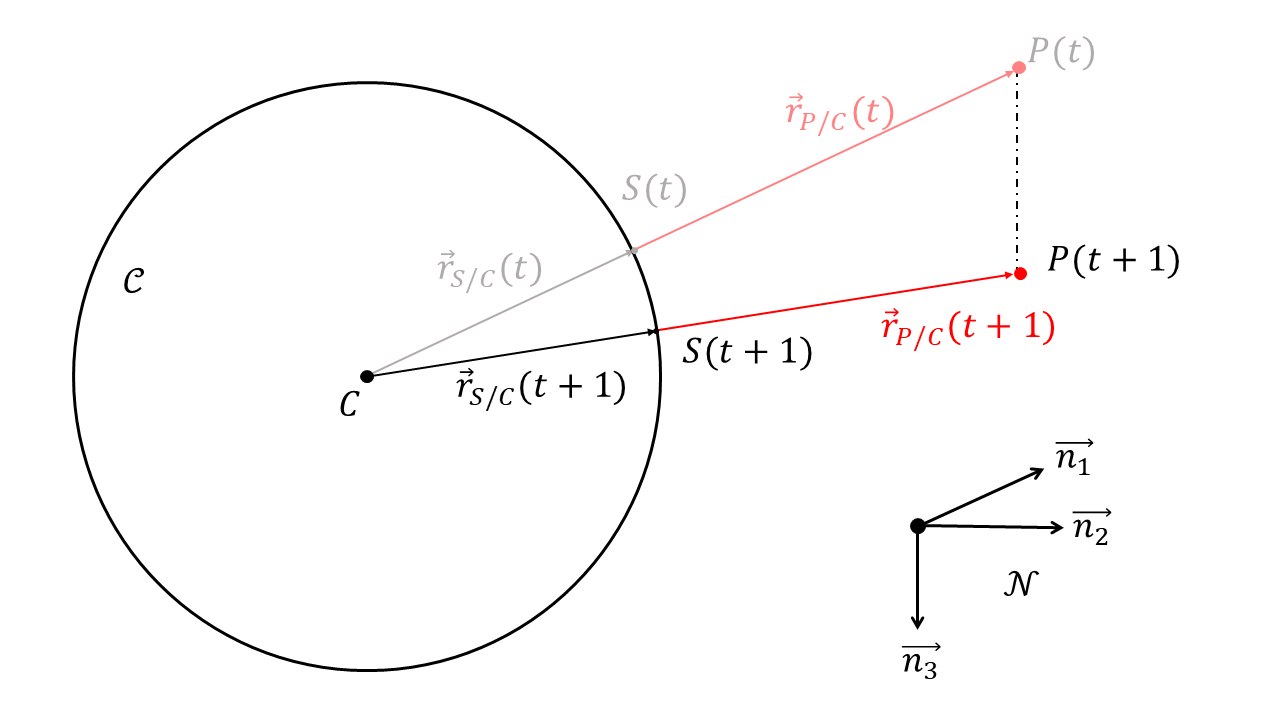
\includegraphics[width=.8\linewidth]{Figures/MeasurementModel}
        \caption{Write something here}
        \label{fig:MeasurementModel}
    \end{center}
\end{figure}
Assuming the viewsphere has a unit radius, the point $P$ can be projected onto the view sphere to point $S$ by:
\begin{equation}
	\vec{r}_{S/C} = \frac{\vec{r}_{P/C}}{\norm{\vec{r}_{P/C}}}
\end{equation}
Applying the concepts from \ref{sec:VectorDerivitives}, the time derivitive of $\vec{r}_{S/C}$ with respect to reference frame $\mathcal{N}$ can be taken: 
\begin{equation}
	\begin{split}
		\frac{{}^\mathcal{N}d\vec{r}_{S/C}}{dt} &= \frac{{}^\mathcal{N}d}{dt}\left(\frac{\vec{r}_{P/C}}{\norm{\vec{r}_{P/C}}}\right)\\
		&= \frac{{}^\mathcal{N}d}{dt}\vec{r}_{P/C}(\vec{r}_{P/C} \cdot \vec{r}_{P/C})^{-\frac{1}{2}}\\
		&=\frac{{}^\mathcal{N}d}{dt}\left(\vec{r}_{P/C}\right)(\vec{r}_{P/C} \cdot \vec{r}_{P/C})^{-\frac{1}{2}} + \vec{r}_{P/C}\frac{{}^\mathcal{N}d}{dt}(\vec{r}_{P/C} \cdot \vec{r}_{P/C})^{-\frac{1}{2}}\\
		&=\frac{\vec{v}_{P/C}}{\norm{\vec{r}_{P/C}}} - \frac{1}{2} \vec{r}_{P/C}(\vec{r}_{P/C}\cdot\vec{r}_{P/C})^{-\frac{3}{2}}\frac{{}^\mathcal{N}d}{dt}(\vec{r}_{P/C} \cdot \vec{r}_{P/C})\\
		&=\frac{\vec{v}_{P/C}}{\norm{\vec{r}_{P/C}}} - \frac{1}{2} \vec{r}_{P/C}(\vec{r}_{P/C}\cdot\vec{r}_{P/C})^{-\frac{3}{2}}\left(2\vec{r}_{P/C}\frac{{}^\mathcal{N}\vec{r}_{P/C}}{dt}\right)\\
		&=\frac{\vec{v}_{P/C}}{\norm{\vec{r}_{P/C}}} - \frac{\vec{r}_{P/C}(\vec{r}_{P/C}\vec{v}_{P/C})}{\norm{\vec{r}_{P/C}}^{3}}\\
		&=\frac{\vec{v}_{P/C}}{\norm{\vec{r}_{P/C}}} - \frac{\vec{r}_{S/C}\norm{\vec{r}_{P/C}}(\vec{r}_{S/C}\norm{\vec{r}_{P/C}}\vec{v}_{P/C})}{\norm{\vec{r}_{P/C}}^{3}}\\
		\vec{r}_{S/C}&=\frac{\vec{v}_{P/C}}{\norm{\vec{r}_{P/C}}} - \frac{\vec{r}_{S/C}(\vec{r}_{S/C}\vec{v}_{P/C})}{\norm{\vec{r}_{P/C}}}
	\end{split}
\end{equation}
As previously mentioned these calculations were with respect to the world reference frame $\mathcal{N}$. However, spherical flow is measured in the camera reference frame $\mathcal{C}$. Therefore we need to apply the transport theorem (\ref{eq:transportTheorem}) obtaining the velocity of a point $S$ as seen from $\mathcal{C}$
\begin{equation}
	\begin{split}
		\frac{{}^\mathcal{C}d\vec{r}_{S/C}}{dt} &=\frac{\vec{v}_{P/C}}{\norm{\vec{r}_{P/C}}} - \frac{\vec{r}_{S/C}(\vec{r}_{S/C}\vec{v}_{P/C})}{\norm{\vec{r}_{P/C}}} + \vec{r}_{S/C}\times\vec{\omega}_{\mathcal{C}/\mathcal{N}}
	\end{split}
\end{equation}

\subsection{Camera Calibration}\label{sec:Background_cameraCal} %TODO: Pretty good, get someone to read
Computer vision begins with the camera detecting light from a scene. This light has travelled from its source, reflecting from an object, through the camera lens, and is recorded on the image sensor. For these rays of light that make up an image to be useful for representing the real-world, the geometry that transforms these rays from the three-dimensional real world to a two-dimensional image plane must be understood; i.e. the transformation from world coordinates to image coordinates.

The camera calibration process describes the camera with two sets of parameters, namely the intrinsic parameters, and the extrinsic parameters. The intrinsic parameters describe the geometric relationship between the camera model and its projection. And the extrinsic parameters describe the location and orientation or pose, of the camera with respect to the world frame.

This project uses a GoPro Hero 7 to test and verify the calibration routine. This section will cover camera models and outline why a planar model is used for the GoPro. It covers the mathematical tools used to capture the different effects that make our camera imperfect for representing the real world, and how these deviations can be corrercted.
\subsubsection{Camera Models}
The most elementary way of representing a camera is with the pinhole model. Light enters the aperture (pinhole) after reflecting from objects in a scene. For an ideal pinhole camera, only one ray enters the aperture from any point in the scene. The light is then projected onto a surface behind the aperture resulting in an image of the scene that is scaled proportionally to the focal length $f$.

\begin{figure}[ht]
    \begin{center}
        \includegraphics[width=.8\linewidth]{Figures/Pinhole_model}
        \caption{Elementary pinhole model of a camera: In practice, the appeture must be big enough to let light in, allowing a narrow ray of light from each point in the scene blurring the image. Therefore there is a tradeoff between brightness and sharpness.}
        \label{fig:PinholeModel}
    \end{center}
\end{figure}

\Cref{fig:PinholeModel} shows an ideal pinhole camera model and its parameters, where $f$ is the focal length, $Z$ is the distance along the optical axis to an object, $x$ is the size of the projected object and $X$ is the size of the object. For this model, \eqref{eq:pinholeEQ} is the relationship between the projected image and the object
\begin{equation}\label{eq:pinholeEQ}
	\frac{-x}{f} = \frac{X}{Z}
\end{equation}
Due to how light enters the camera, the image projection from a pinhole model is projected upside down. This issue is fixed in a planar camera model. The planar model is similar to a pinhole model, however rather than passing through an aperture, light travels from each point in the scene, intersects the image plane and converges to a single point known as the \textit{centre of projection} \Cref{fig:PlainarModel}. The Plainar Model better represents the geometry of a camera with a lens, albeit a camera with an impossibly perfect lens.

\begin{figure}[ht]
	\begin{minipage}[c]{0.3\linewidth}
		\centering
		\begin{tabular}{l l}
			$C$ &: Centre of projection\\
			$\{c\}$ &: Camera co-ordinates\\
			$P$ &: Point in world space\\
			$P'$ &: Point on image plane\\
			$\vec{u}, \vec{v}$ &: Image co-ordinates\\
			$f$ &: Focal length\\
			$I$ &: Image plane
		\end{tabular}
	\end{minipage}
	\begin{minipage}[c]{0.65\linewidth}
		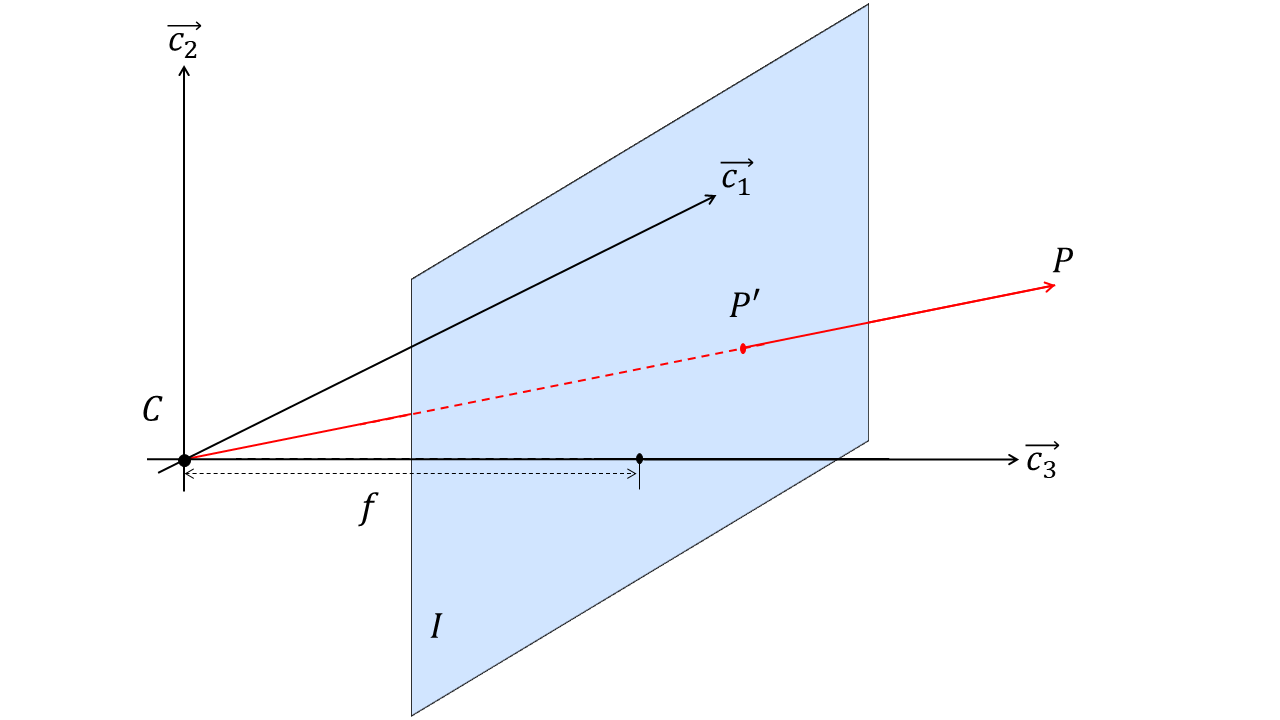
\includegraphics[width=1\linewidth]{Figures/Planar_Model}	
	\end{minipage}
\caption{Ideal camera model. A point $P$ in camera coordinates $(c_{1}, c_{2}, c_{3})$ is projected and displayed as a point $p$ in image co-ordinates $(u, v)$}
\label{fig:PlainarModel}
\end{figure}
The idea behind modelling and calibrating a camera is to identify and cancel out imperfections caused by slight defects in the manufacturing process. Firstly, the image sensor is often mounted out of line from the optical centre of the lens. Therefore, the parameters $u_{0}$ and $v_{0}$ are introduced to model this displacement from the optical centre. Furthermore, each pixel is not necessarily square, causing a small discrepancy between the focal length in the $u$ and $v$ directions. These discrepancy are captured in the $f_{u}$ and $f_{v}$ parameters. The following \Cref{eq:ProjectionEquations} project a point $P_{c_{1}, c_{2}, c_{3}}$ to image sensor co-ordinates $(u, v)$:
\begin{equation}\label{eq:ProjectionEquations}
	\begin{split}
		u = &f_{u} \times \frac{c_{1}}{c_{3}} + u_{0}\\
		v = &f_{v} \times \frac{c_{2}}{c_{3}} + v_{0}
	\end{split}
\end{equation}
\subsubsection{Projective Geometry}
Projective geometry is a tool describing the relationship that transforms a point from world coordinates $(n_1, n_2, n_3)$ into image coordinates $(u, v)$. When applying such transformations, it is convenient to add an extra dimension to each vector in the transform. for instance, a point that lies in a $n$ dimensional space is represented as a $n+1$ dimensional vector. this coordinate system is known as \textit{homogeneous coordinates}. for example, a point lying on a plane at $(x, y)$ is represented by the homogeneous coordinates $(x, y, z)$. It is important to note that in homogeneous coordinates, any two vectors that share a common factor represents the same point in Euclidean geometry. This has the effect that a point in Euclidean geometry can be represented by an infinite number of homogeneous vectors. for instance $\alpha * (q_{1}, q_{2}, q_{3}) \equiv (q_{1}, q_{2}, q_{3})$. The original primitive point is recovered by dividing through by $q_{3}$.

the utility of homogenious coordinates becomes clear when common transformations such as translation, rotation and scailing are attempted in . Homogenious coordinates allow these transformations to be implemented with matrix opperations. This is how projective geometry allows the camera intrinsic parameters $f_{u}, f_{v}, u_{0}, v_{0}$ to be arranges into a single $3\times3$ \textit{camera intrinsic matrix} matrix. Bringing all of thees concepts together, the \Cref{eq:ProjectionEquations} can be implemented as a single martix opperation of the form:

\begin{equation}
	p = \mathbf{M}\mathbf{r}^{C}_{P/C}
\end{equation}
where:
\begin{equation}\label{eq:CameraMatrix}
	P = 
    \begin{bmatrix}
        u\\
        v\\
        w
	\end{bmatrix},
	M = 
	\begin{bmatrix}
        f_{u} & 0 & u_{0}\\
        0 & f_{v} & v_{0}\\
        0 & 0 &1
	\end{bmatrix}
	\textrm{and } \mathbf{r}^{C}_{P/C} = 
	\begin{bmatrix}
        c^{c}_{1}\\
        c^{c}_{2}\\
        c^{c}_{3}
	\end{bmatrix}
\end{equation}
Some older camera manufacturing processes produce nonrectangular image sensors, i.e. they produced parallelogram shaped sensors. To account for this, a final \textit{skew} parameter was included. Most modern cameras are produced with close to no skew therefor the error that this effect causes is below the noise floor and assumed to be $0$.
\subsubsection{Lens Distortion}
The optics inside a camera are yet another source of error in an image. Similar to correcting for the cameras geometry (captured in \ref{eq:CameraMatrix}), lens distortion must be accounted for. The leading method for correcting Lens distortion uses a \textit{Brown-Conrady model} from \cite{fryer1986lens}. This model characterises the two most prominent sources of distortion, naimley \textit{radianl distortion} and \textit{tangental distortion} and undistorts the image pixel locations.

In an ideal camera, the lense would take the shape of a perfect paraboloid. However it is much easier and cheeper to produce a sperical lens. The spherical shape of the lens tends to "over bend" rays entering farther from the optical center producing the effect known as \textit{Radial Distortion} \cref{fig:RadialDistortion}. Typically a taylor series is used to characterise the distortion caused by the lens \cite{learningOpenCV}. This polynomial takes the form:
\begin{equation}
	f(r) = a_{0} + a_{1}r + a_{2}r + a_{3}r\dots
\end{equation}
where $r = \sqrt{u^{2} + v^{2}}$ is the radial distance from the optic centre.

\begin{figure}[ht]
	\subfloat[][Red - "spherical" lens

				Blue - paraboloidal lens]
				{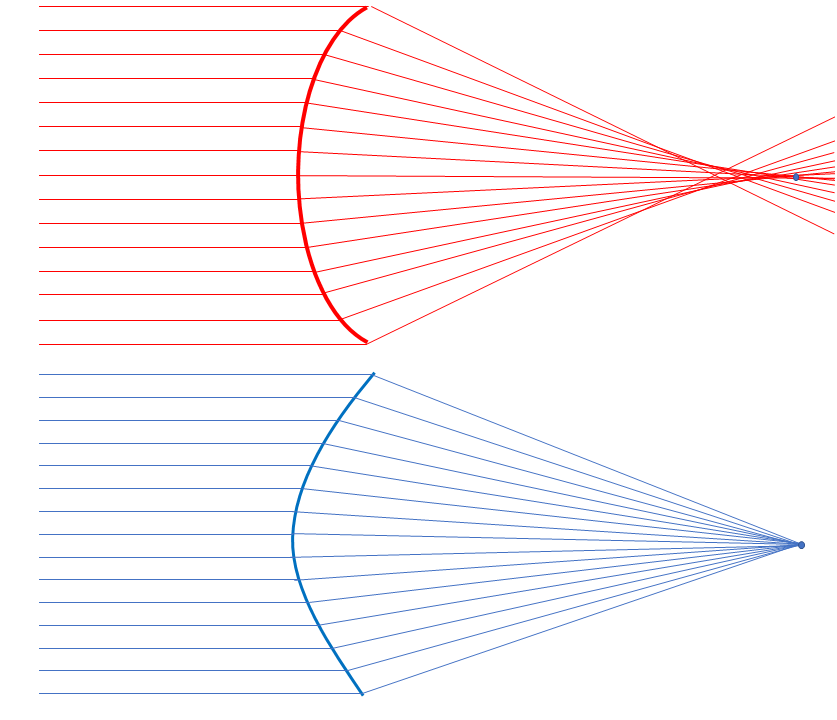
\includegraphics[width=.35\linewidth]{Figures/ParabolicLens}}
	\subfloat[Radial distortion is most clear on square objects]{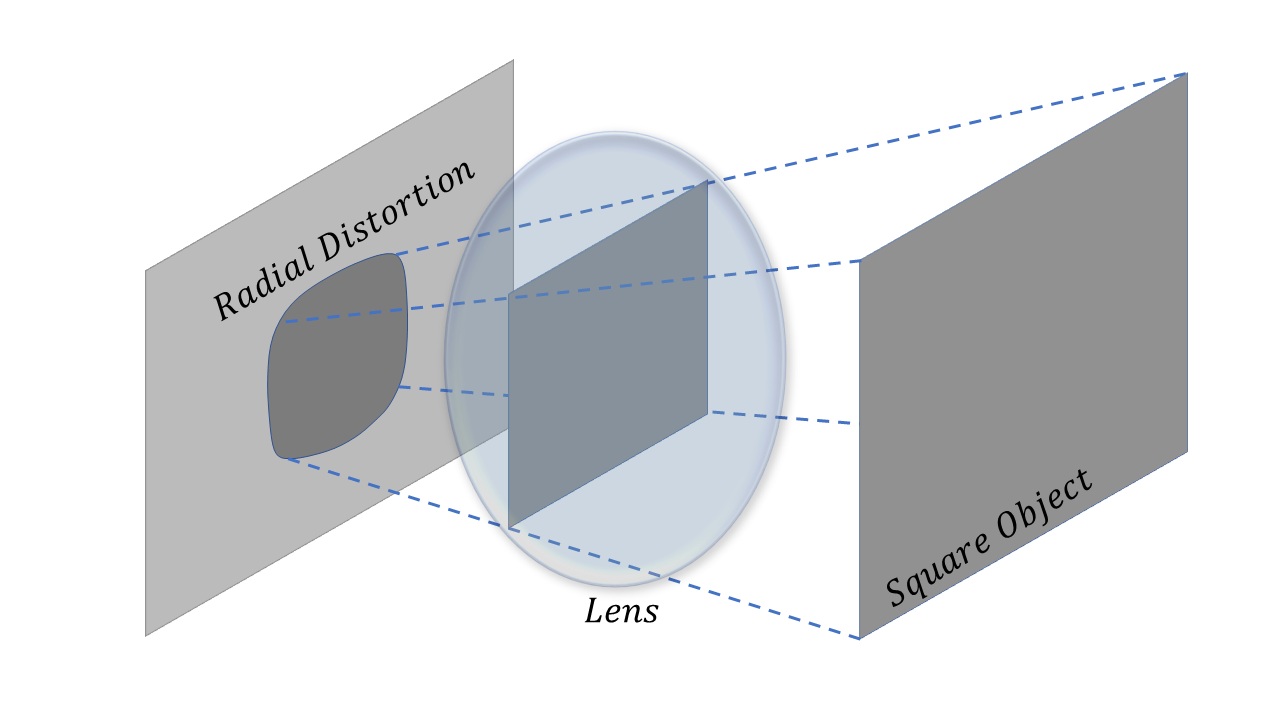
\includegraphics[width=.6\linewidth]{Figures/RadialDistortion}}
	\caption{Radial distortion also known as \textit{Barrel Distortion}. The farther from the centre a ray enters, the larger the barrel distortion bends it.}	
	\label{fig:RadialDistortion}
\end{figure}

However, for radial distortions, at the optical centre of the lense, deviation cause to the light rays is minimal i.e. $f(r) = 0$ at $r = 0$. This further implies that $a_0 = 0$. Additionally, becaues the distortion must be symetrical in $r$, the coefficents of the odd powers of $r$ equal $0$. This means that only the parameters needed for radial distortion correction are the coefficents of even powers of $r$ \cite{learningOpenCV}. Typically, no more than three radial distortion parameters $(k_{1}, k_{2}, k_{3})$ are needed. However, for high \textit{field of view} cameras, upto $K_{6}$ may be necessary. Once these parameters are found, each pixel will be rescaled according to the following equations:
\begin{equation}\label{eq:radialParameters}
	\begin{split}
	u' = u\times(1+k_{1}r^{2} + k_{2}r^{4} + k_{3}r^{6})\\
	v' = v\times(1+k_{1}r^{2} + k_{2}r^{4} + k_{3}r^{6})
	\end{split}
\end{equation}
where $u'$ and $v'$ are the undistorted pixel coordinates.

Not only is it expensive and dificult to produce a lens that perfectly trains rays of light onto the \textit{centre of projection} of a camera, it is also dificult to mechanically mount the image sensor to the camera body such that it is parallel to the lense.

\begin{figure}[ht]
	\subfloat[Ray diagram of tangental distortion]{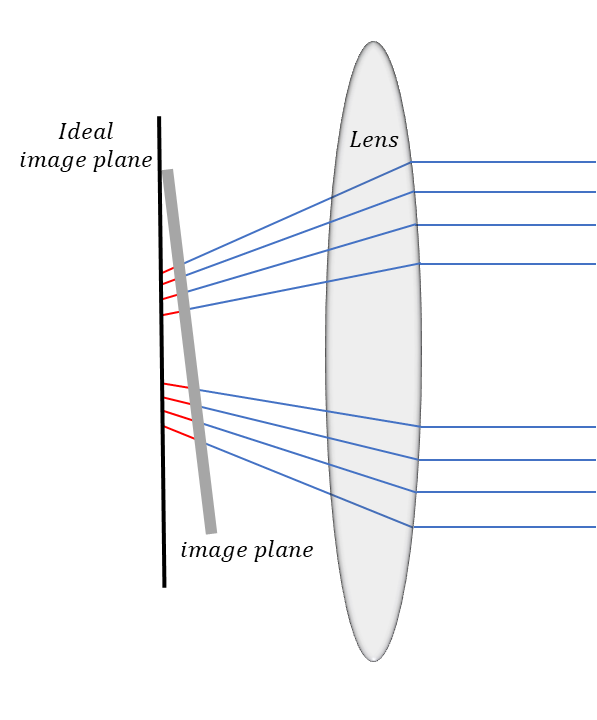
\includegraphics[width=.4\linewidth]{Figures/tangentalDistortion}}
	\subfloat[Tangental distortion of a flat grid]{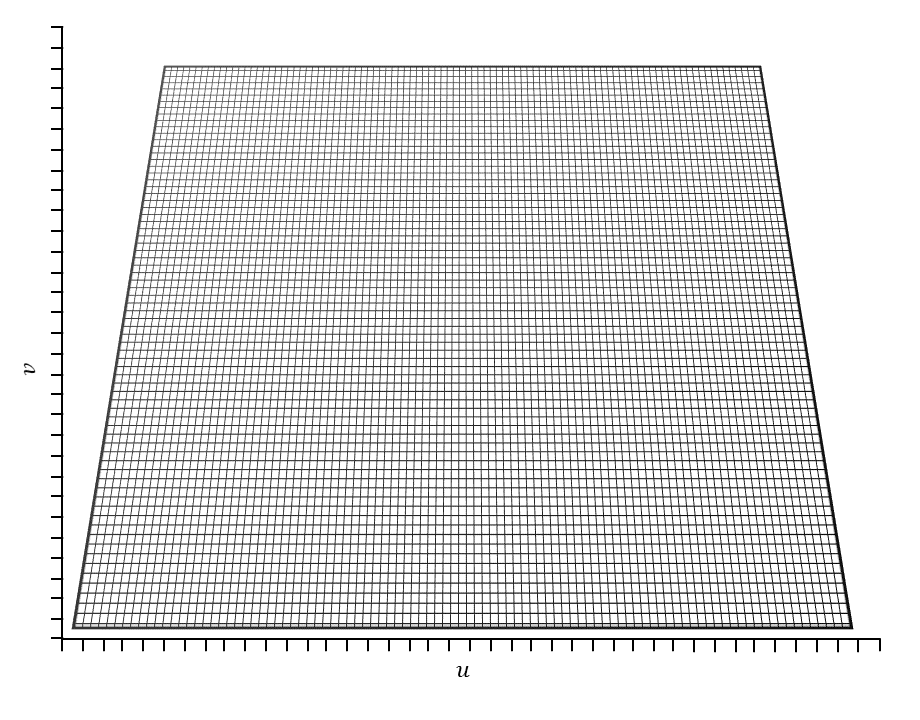
\includegraphics[width=.6\linewidth]{Figures/tangentalImage}}
	\caption{Extream example of tangental distortion.}	
	\label{fig:RadialDistortion}
\end{figure}

Two additional parameters $p_{1}$ and $p_{2}$ are introduced to minimally characterise this tangental distortion such that:

\begin{equation}\label{eq:tangentalParameters}
	\begin{split}
		u' &= u + [2p_{1}uv + p_{2}(r^{2} + 2u^{2})]\\
		v' &= v  + [p1(r^{2} + 2v^2) + 2p_{2}uv]
	\end{split}
\end{equation}
There are many other aspects within an average camera that cause image distortion, howerver these effects contribute a minor amount to the accuracy of measurements from an image so for this project will be assumed $0$. Both Matlab and Open CV based camera calibration rotines are implemented and evaluated in this project. The camera calibration routine for Matlab \textit{estimateCameraParameters();} returns an object containing the camera matrix \ref{eq:CameraMatrix}, radial distortion parameters \ref{eq:radialParameters} and tangental distortion parameters \ref{eq:tangentalParameters}, along with information about the calibration photos. When using \textit{Open CV}, these parametetrs are packaged into a \textit{distortion vector}. For this project, six radial distortion parameters were used to capture the distortion for a Go Pro Hero 7. Therefor the distortion vector from Open CV is organised as $(k_{1}, k_{2}, p_{2}, p_{1}, k_{3}, k_{4}, k_{5}, k_{6})$.
From \cref{eq:radialParameters} and \cref{eq:tangentalParameters}, the \textit{Brown-Conrady model} is as follows:
\begin{equation}
	\begin{split}
		u' &= u\left(\frac{1  +k_{1}r^{2} + k_{2}r^{4} + k_{3}r^{6}}{k_{4}r^{2} + k_{5}r^{4} + k_{6}r^{6}}\right) + 2p_{1}uv + p_{2}(r^{2} + 2u^{2})\\
		v' &= v\left(\frac{1  +k_{1}r^{2} + k_{2}r^{4} + k_{3}r^{6}}{k_{4}r^{2} + k_{5}r^{4} + k_{6}r^{6}}\right)  + p_{1}(r^{2} + 2v^{2}) + 2p_{2}uv\\
	\end{split}
\end{equation}
Now that the camera can be discribed mathmatically through the intrinsic parameters and distorion parameters, pixel location in the image can be \textit{undistorted}. \Cref{fig:DistortionMovement} shows the movement of a subset of pixes from a GoPro Hero 7 image. Notice the movement of pixels in the centre of the image move far less than thoes radialy further away.
\begin{figure}[ht]
    \begin{center}
        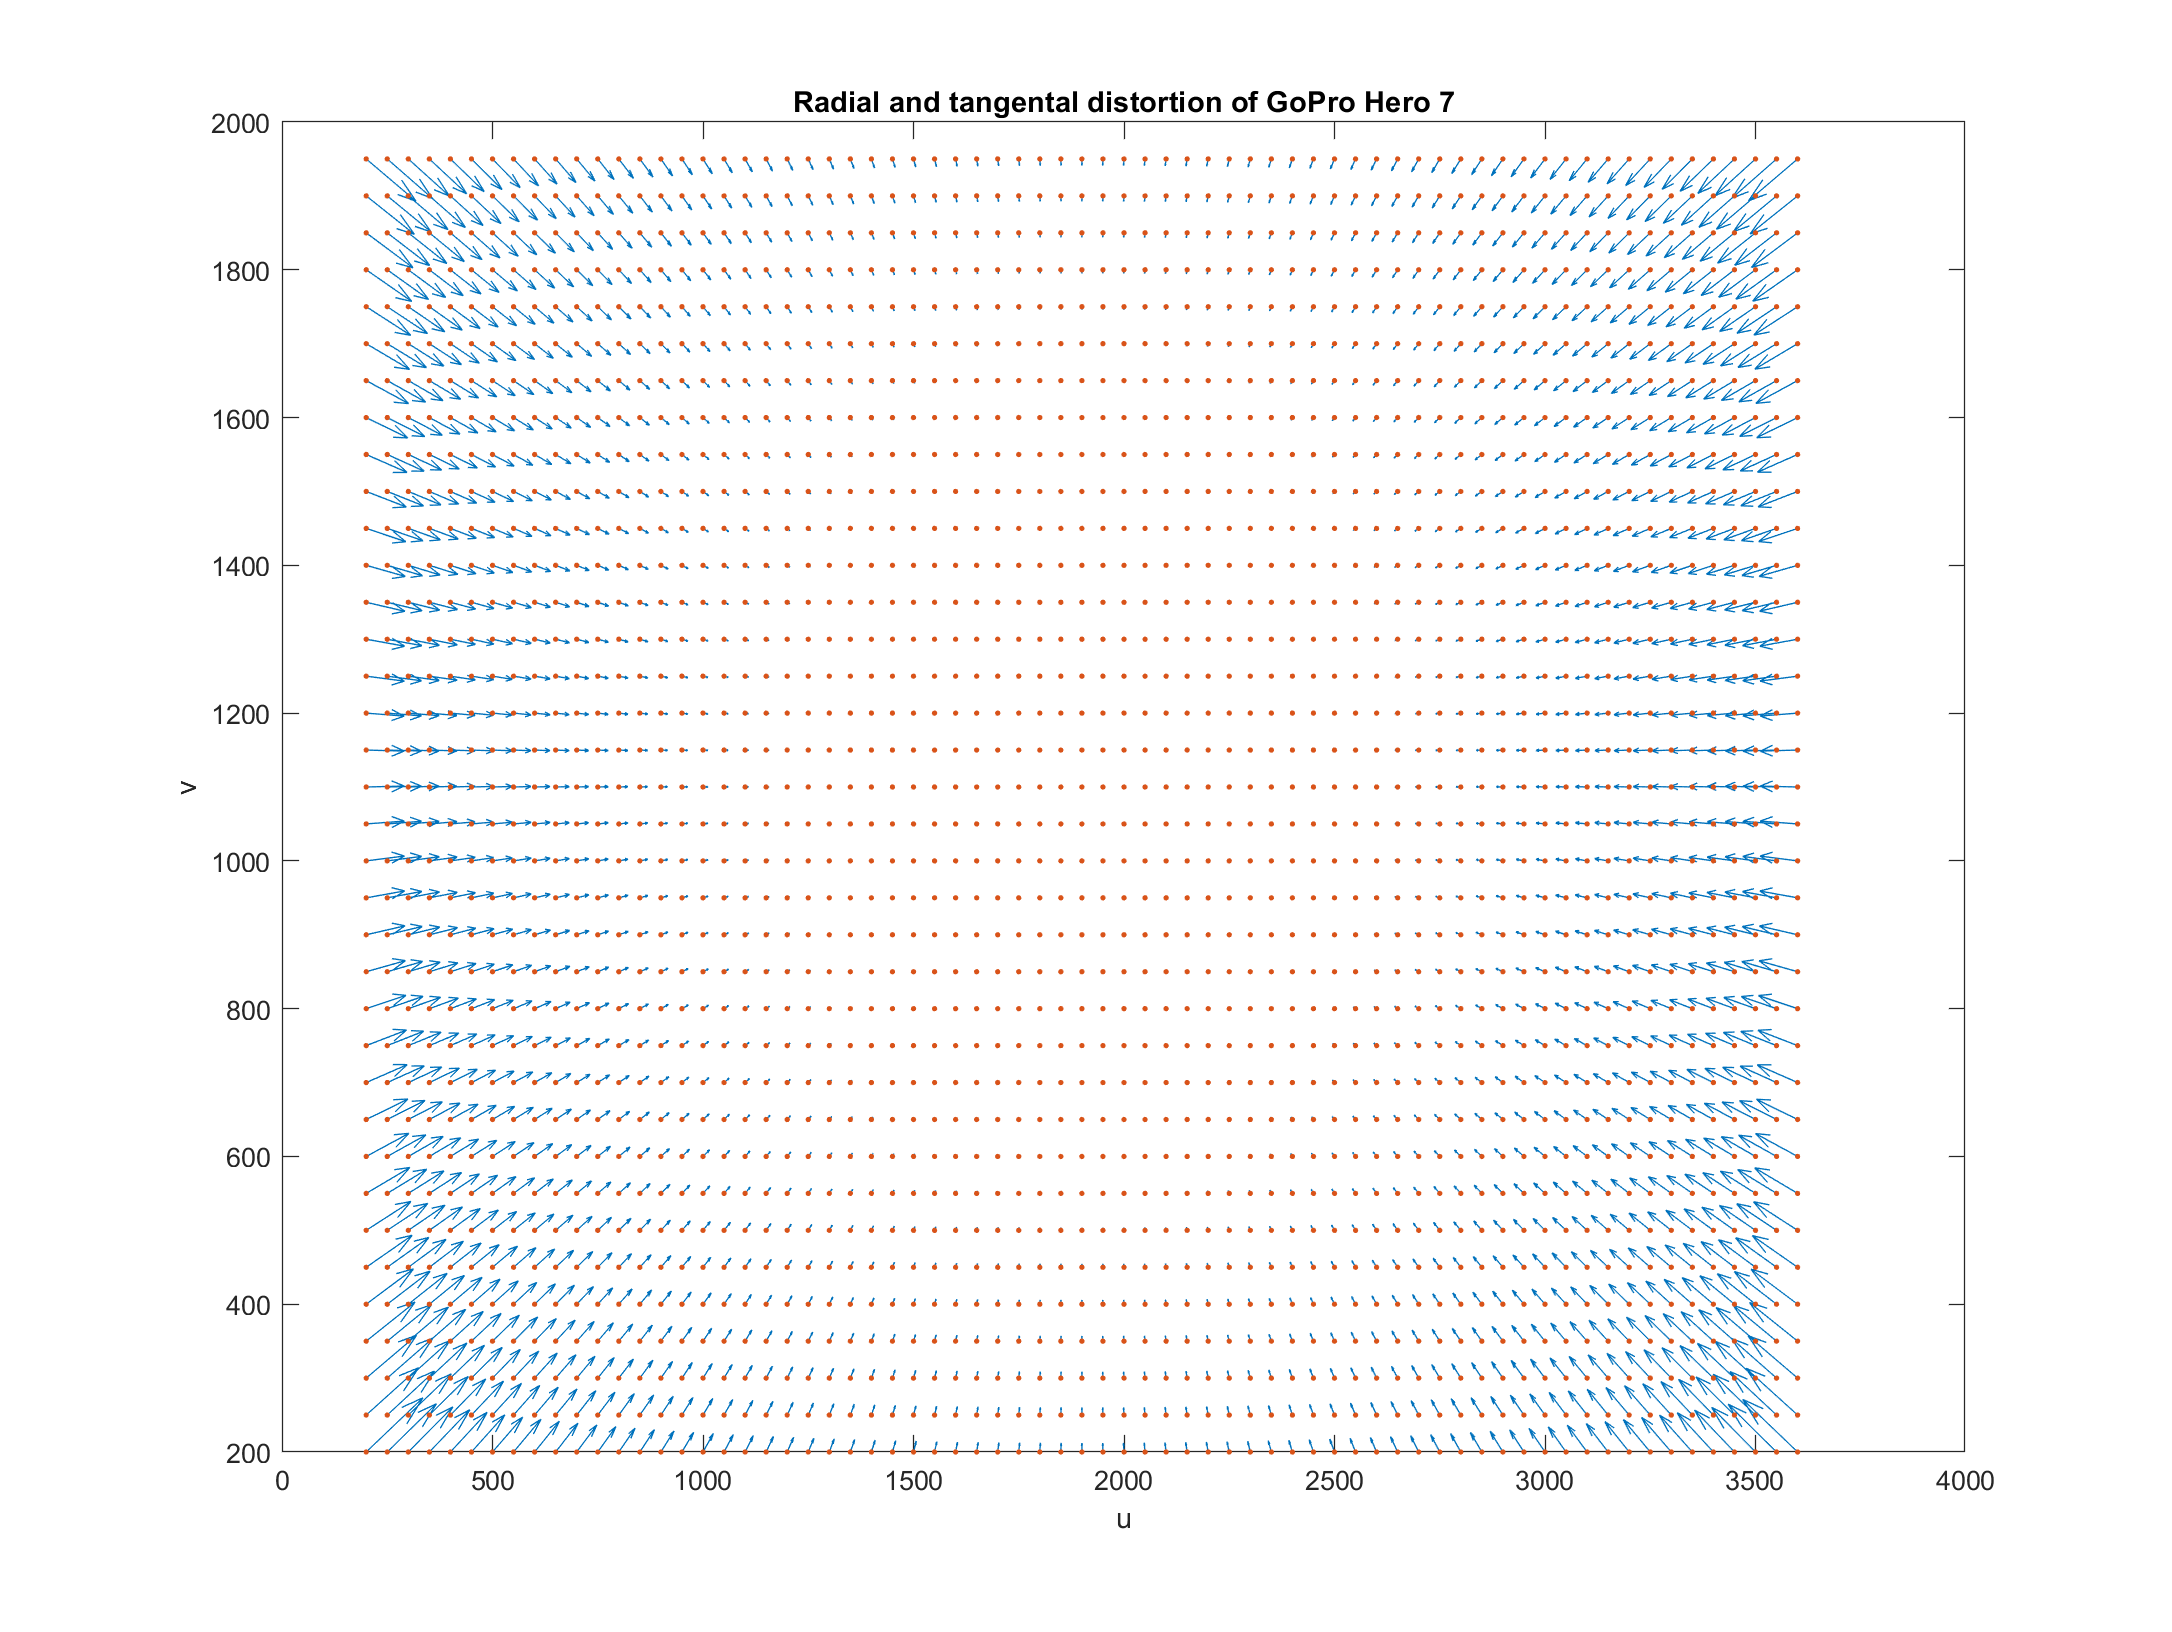
\includegraphics[width=.9\linewidth]{Figures/Matlab/DistortionMovement}
        \caption{Shows the movement of a sample of pixels based on the parameters of a GoPro}
        \label{fig:DistortionMovement}
    \end{center}
\end{figure}
\subsection{Trajectorie Planning}

%%%%%%%%%%%%%%%%%%%%%%%%%%%%%%%
\newpage
\section{Data simulation and Collection}
Simulating the model discussed in 
The project is primaritly simmulation based. However, the camera calibration routine (explored in following sections was tested and evaluated on real world images collected from a GoPro Hero 7. Were this project to be implemented on a real world fixed wing UAV, the kinematic data would need to be obtained through sensors on the UAV.

%%%%%%%%%%%%%%%%%%%%%%%%%%%%%%%
\newpage
\section{Optical Flow - Simulation}
As discussed in sing the spherical flow model discribed in \ref{sec:SphericalFlow}

\begin{figure}[ht]
    \begin{center}
        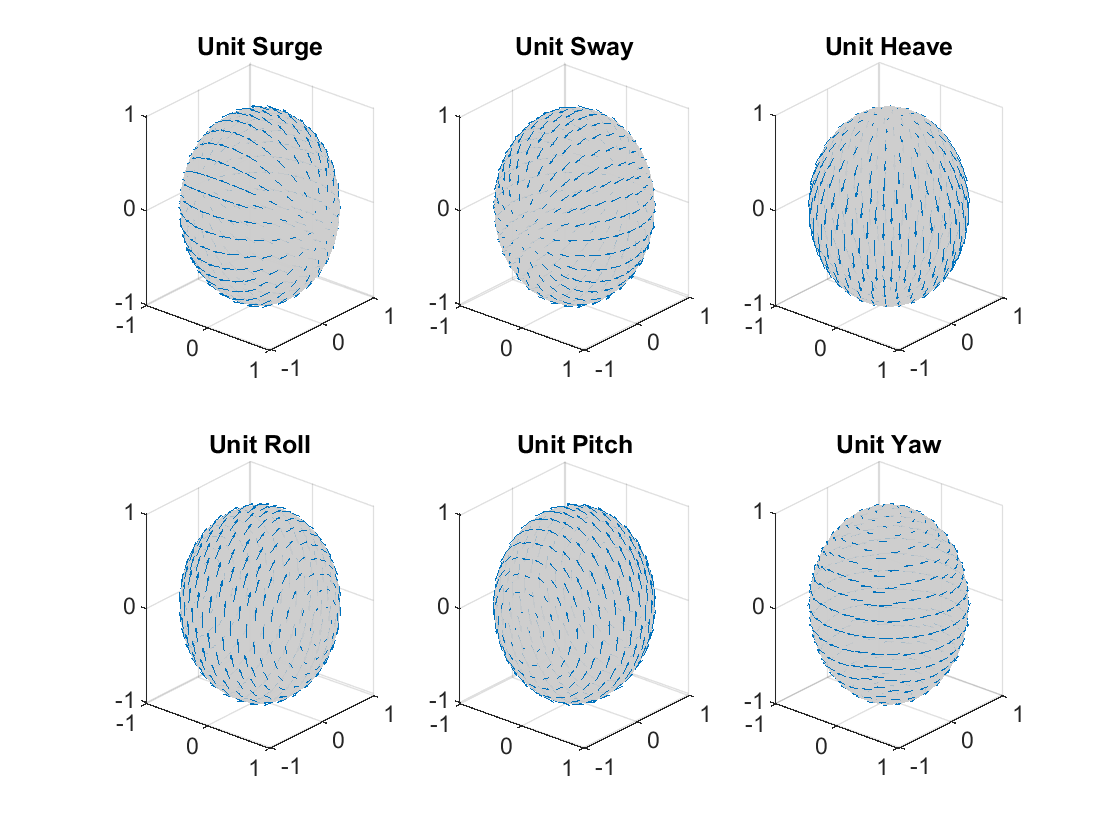
\includegraphics[width=.6\linewidth]{Figures/Unit_Movement}
        \caption{Write something here}
        \label{fig:Unit_Movement}
    \end{center}
\end{figure}
\subsection{Measurement Model}
\begin{figure}[ht]
    \begin{center}
        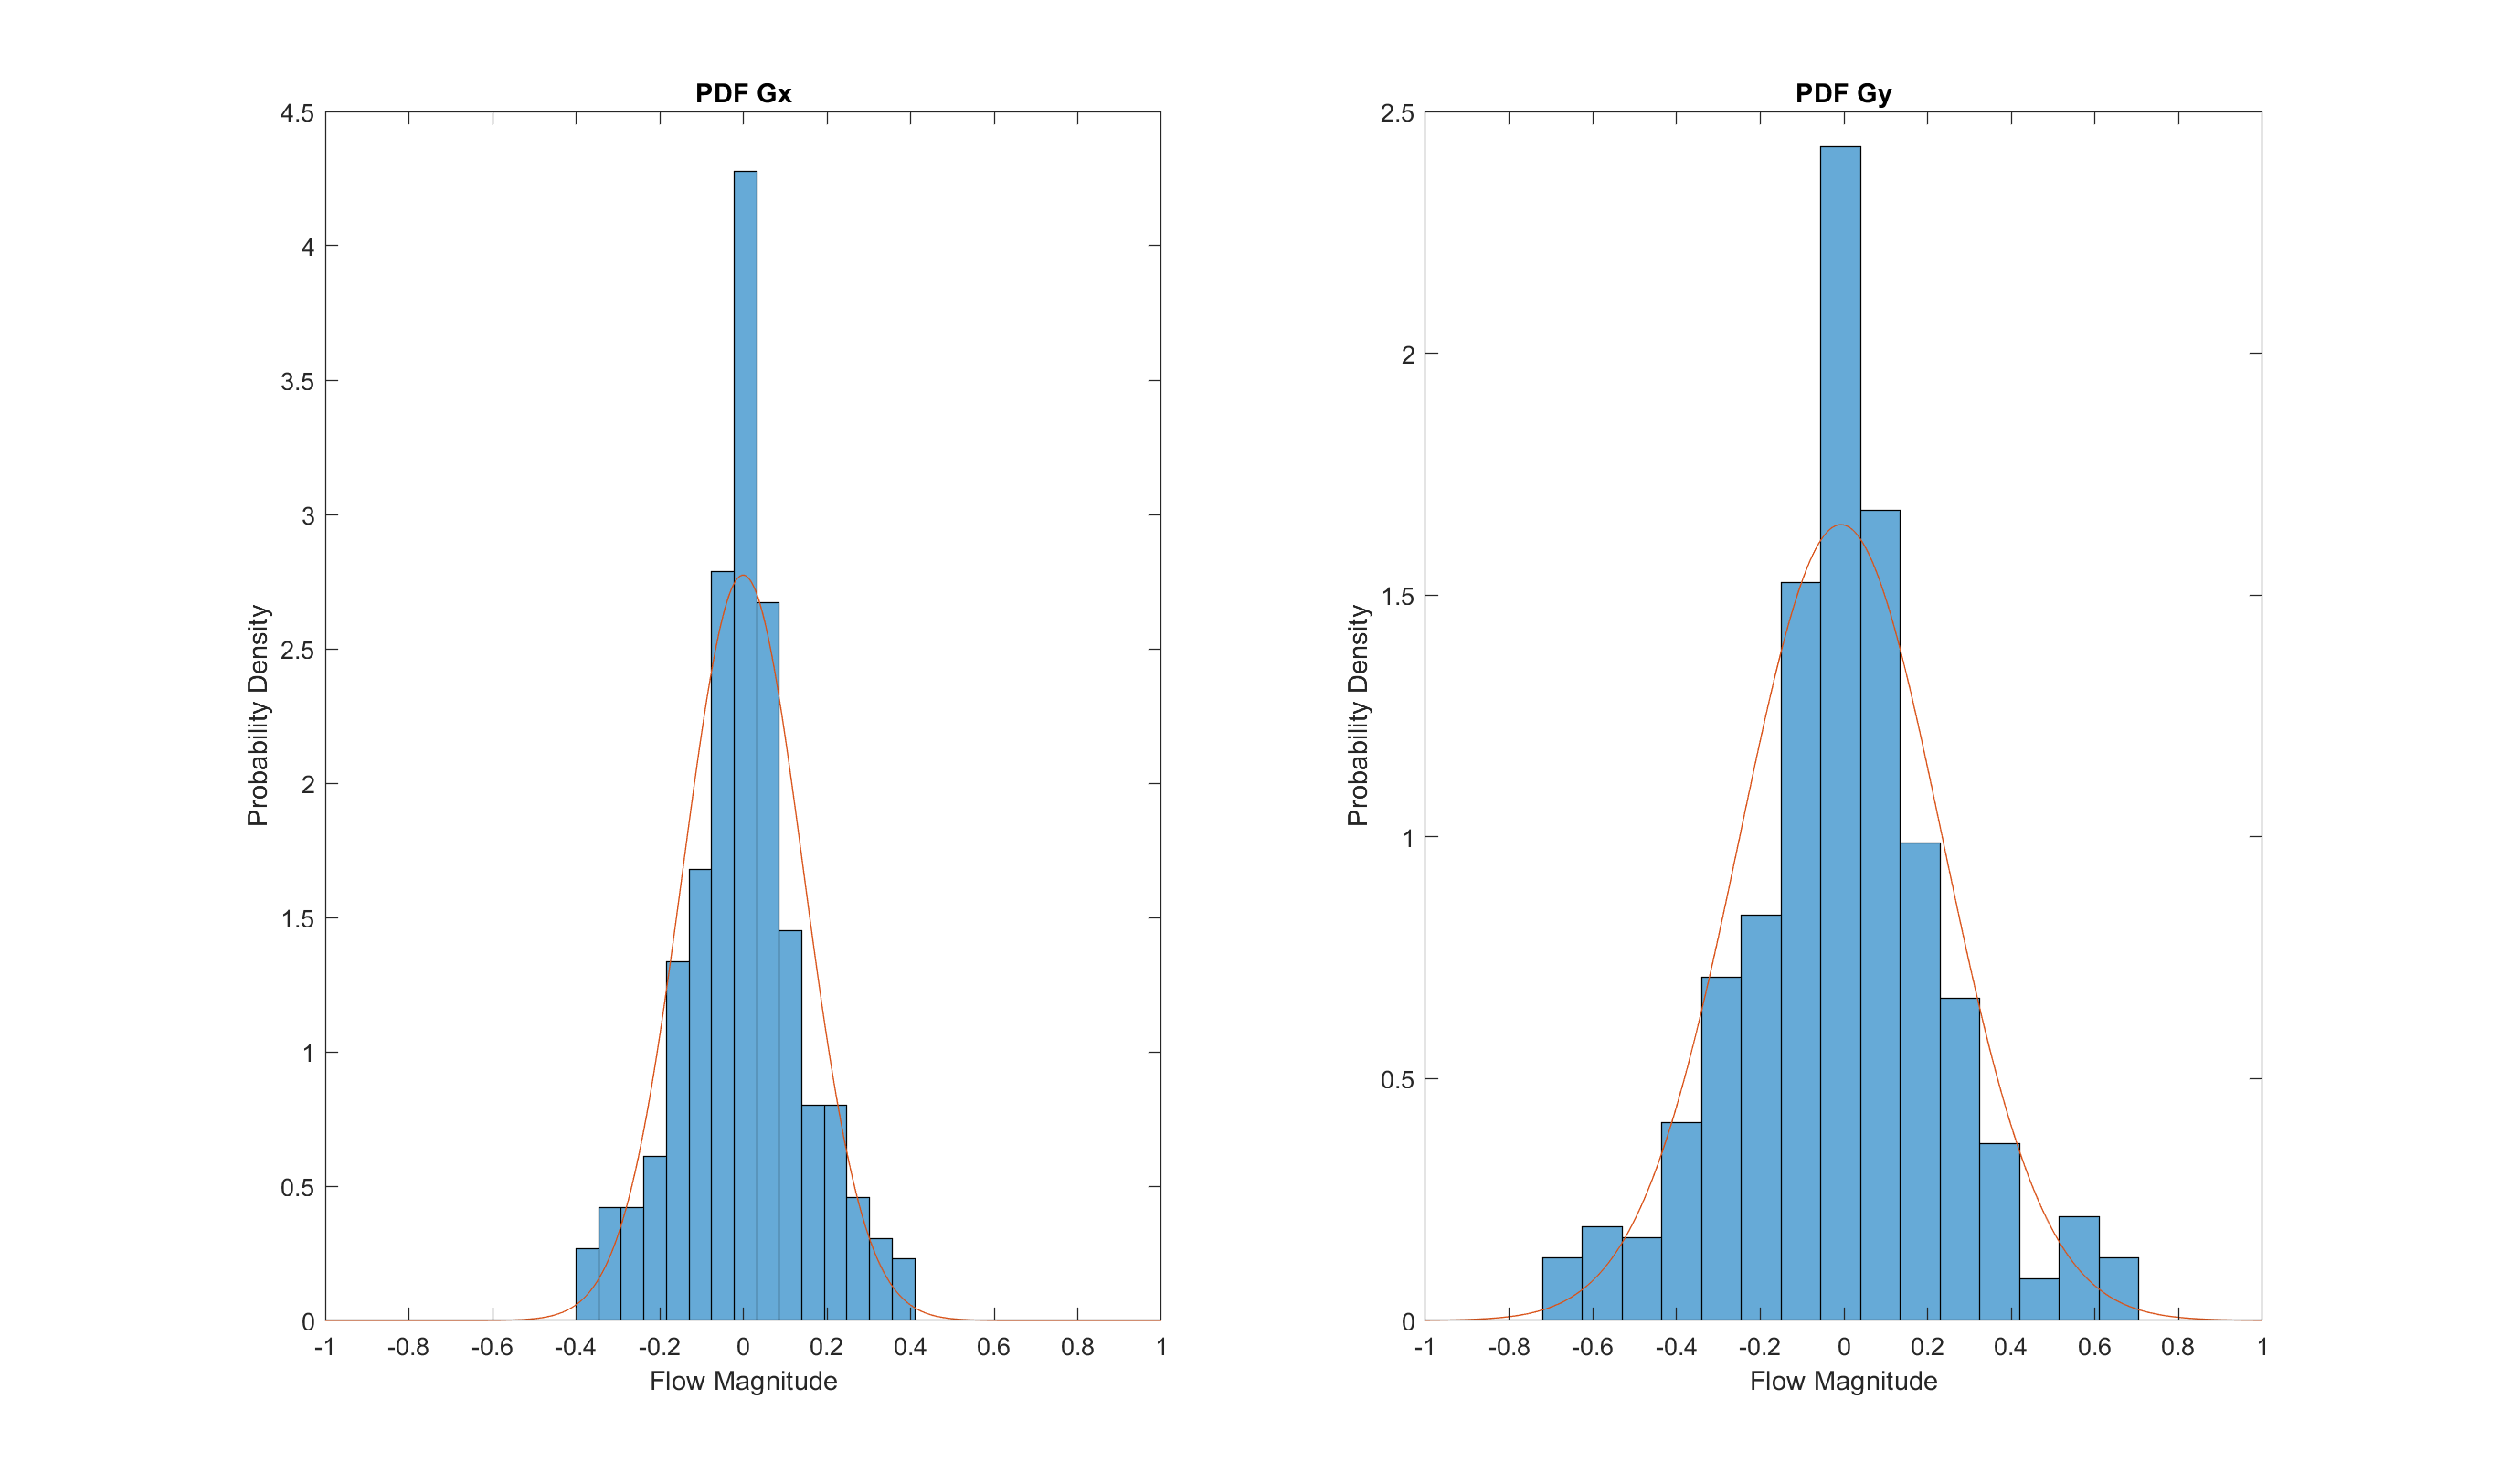
\includegraphics[width=.6\linewidth]{Figures/Matlab/GoPro_Noise_PDF}
        \caption{Write something here}
        \label{fig:GoPro_Noise_PDF}
    \end{center}
\end{figure}
\subsection{Farnback Algorithm - OpenCV}

\newpage
\section{Camera Calibration}
As discussed in \Cref{sec:Background_cameraCal} it is imperitive to understand and account for the construction and imperfections in a camera, if the measurments taken need to be relevent outside image coordinates. This section outlines the procedure used in this project to correct a GoPro hero 7 using a planar camera model and a 6th order equation to correct for distortion parameters.
\subsection{Calibration Boards}
Theoretically, to calibrate a camera any object could be used as a calibration object, so log as it is appropriately characterised. However it is much more practical to use a well defined and easily defined object. For this reason, a flat rigid checker pattern was chosen. The geometry of the calibration pattern can be seen in \Cref{fig:cornerLocations}

\begin{figure}[ht]
    \begin{center}
        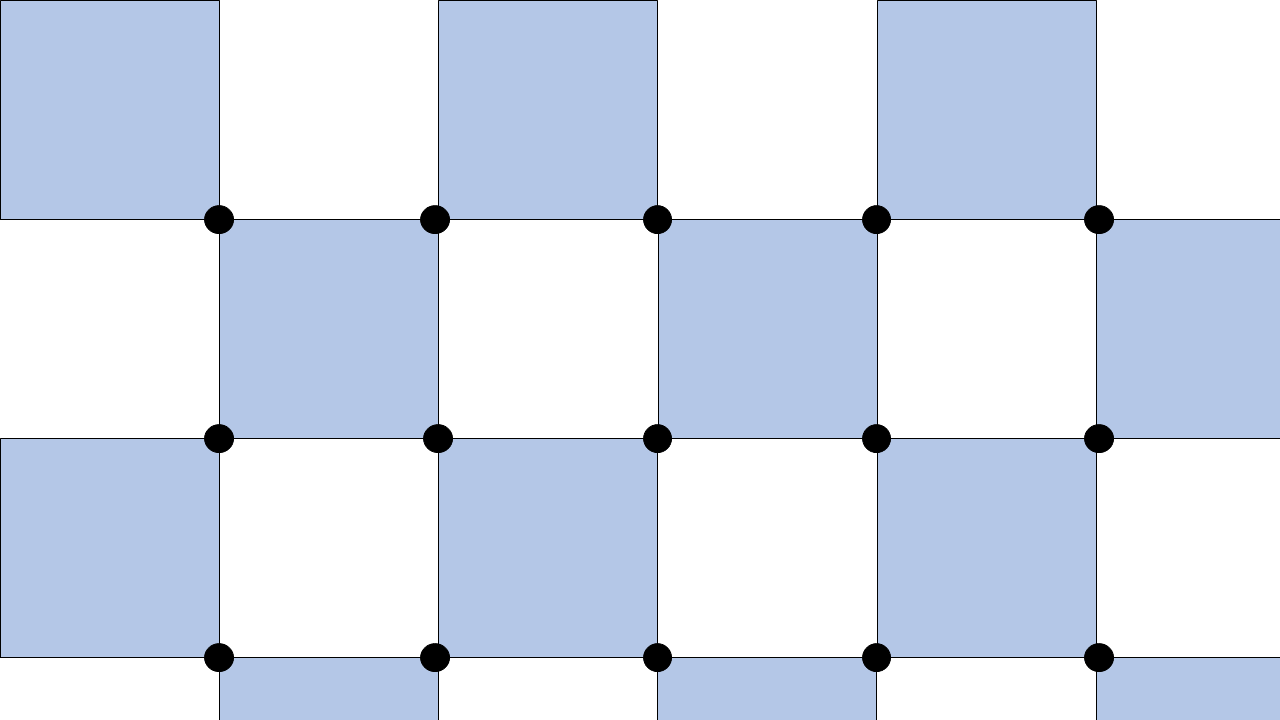
\includegraphics[width=.6\linewidth]{Figures/CalibCornerLocations}
        \caption{Write something here}
        \label{fig:cornerLocations}
    \end{center}
\end{figure}


\subsection{Calibration Tool}
To calibrate the GoPro Hero 7 for in this project, A camera calibration tool was written in C\# using WPF as a graphical user interface(see \Cref{app:calibrationTool})). 
\subsection{Calibration Results}
\begin{figure}[ht]
    \begin{center}
        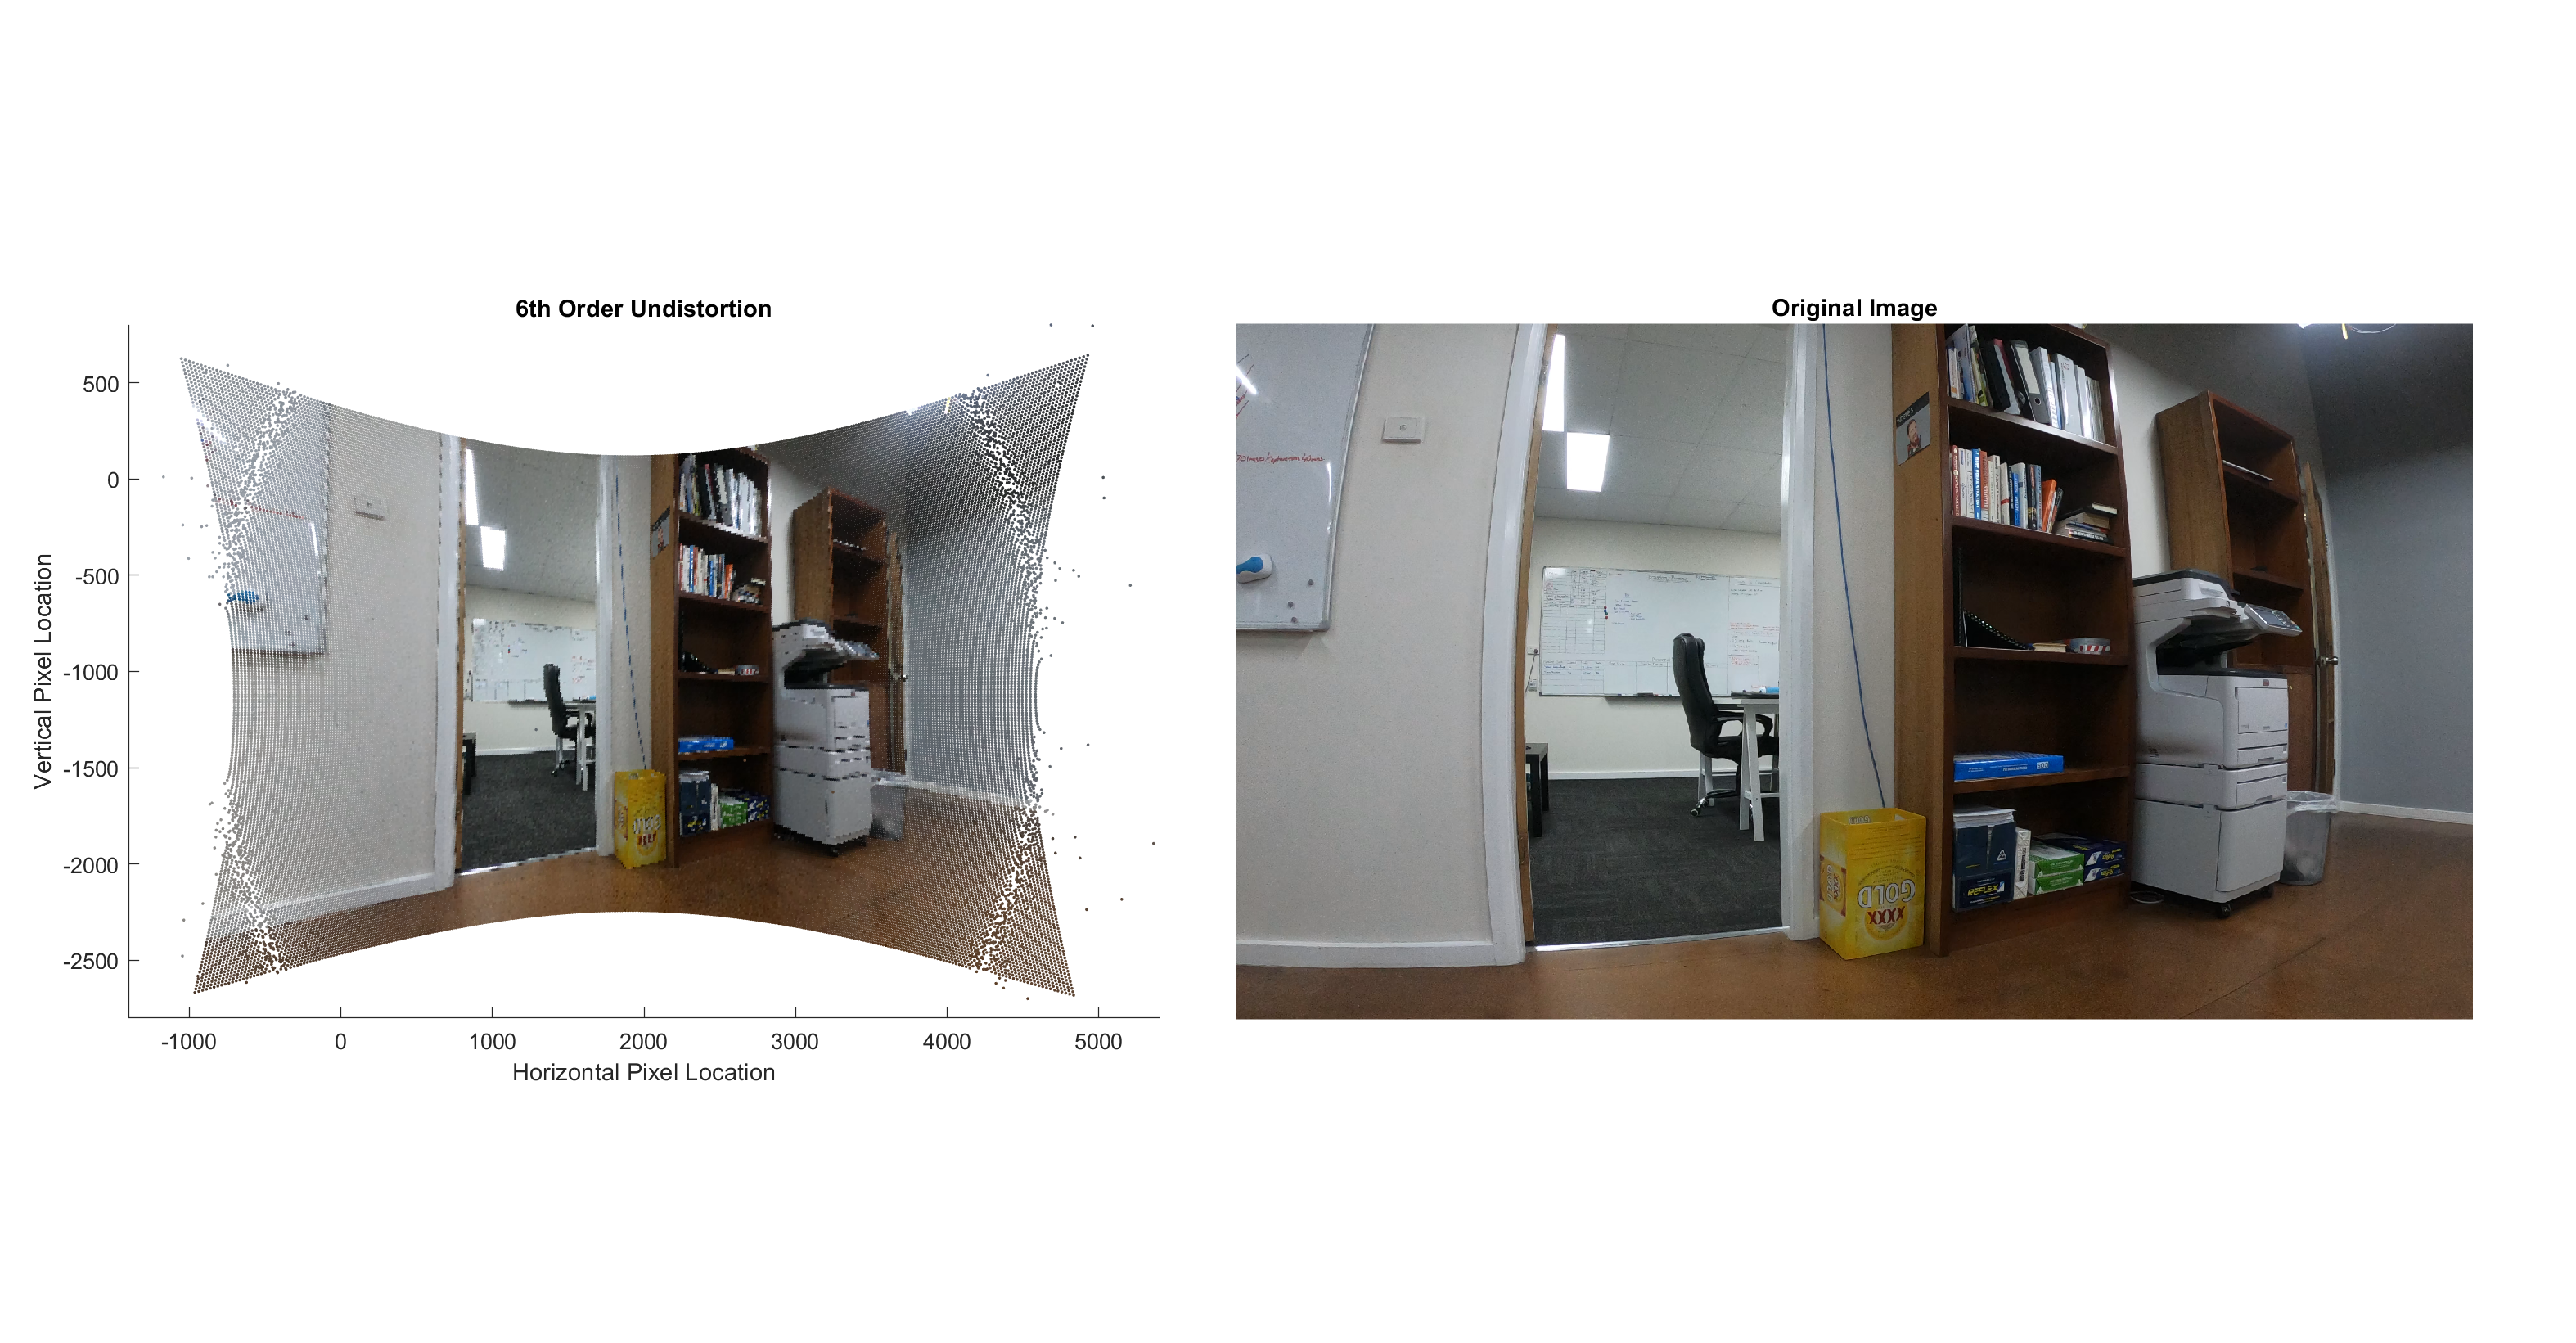
\includegraphics[width=.8\linewidth]{Figures/Matlab/6rdOrderUndistort}
        \caption{Caption}
        \label{fig:6rdOrderUndistort}
    \end{center}
\end{figure}
\begin{figure}[ht]
    \begin{center}
        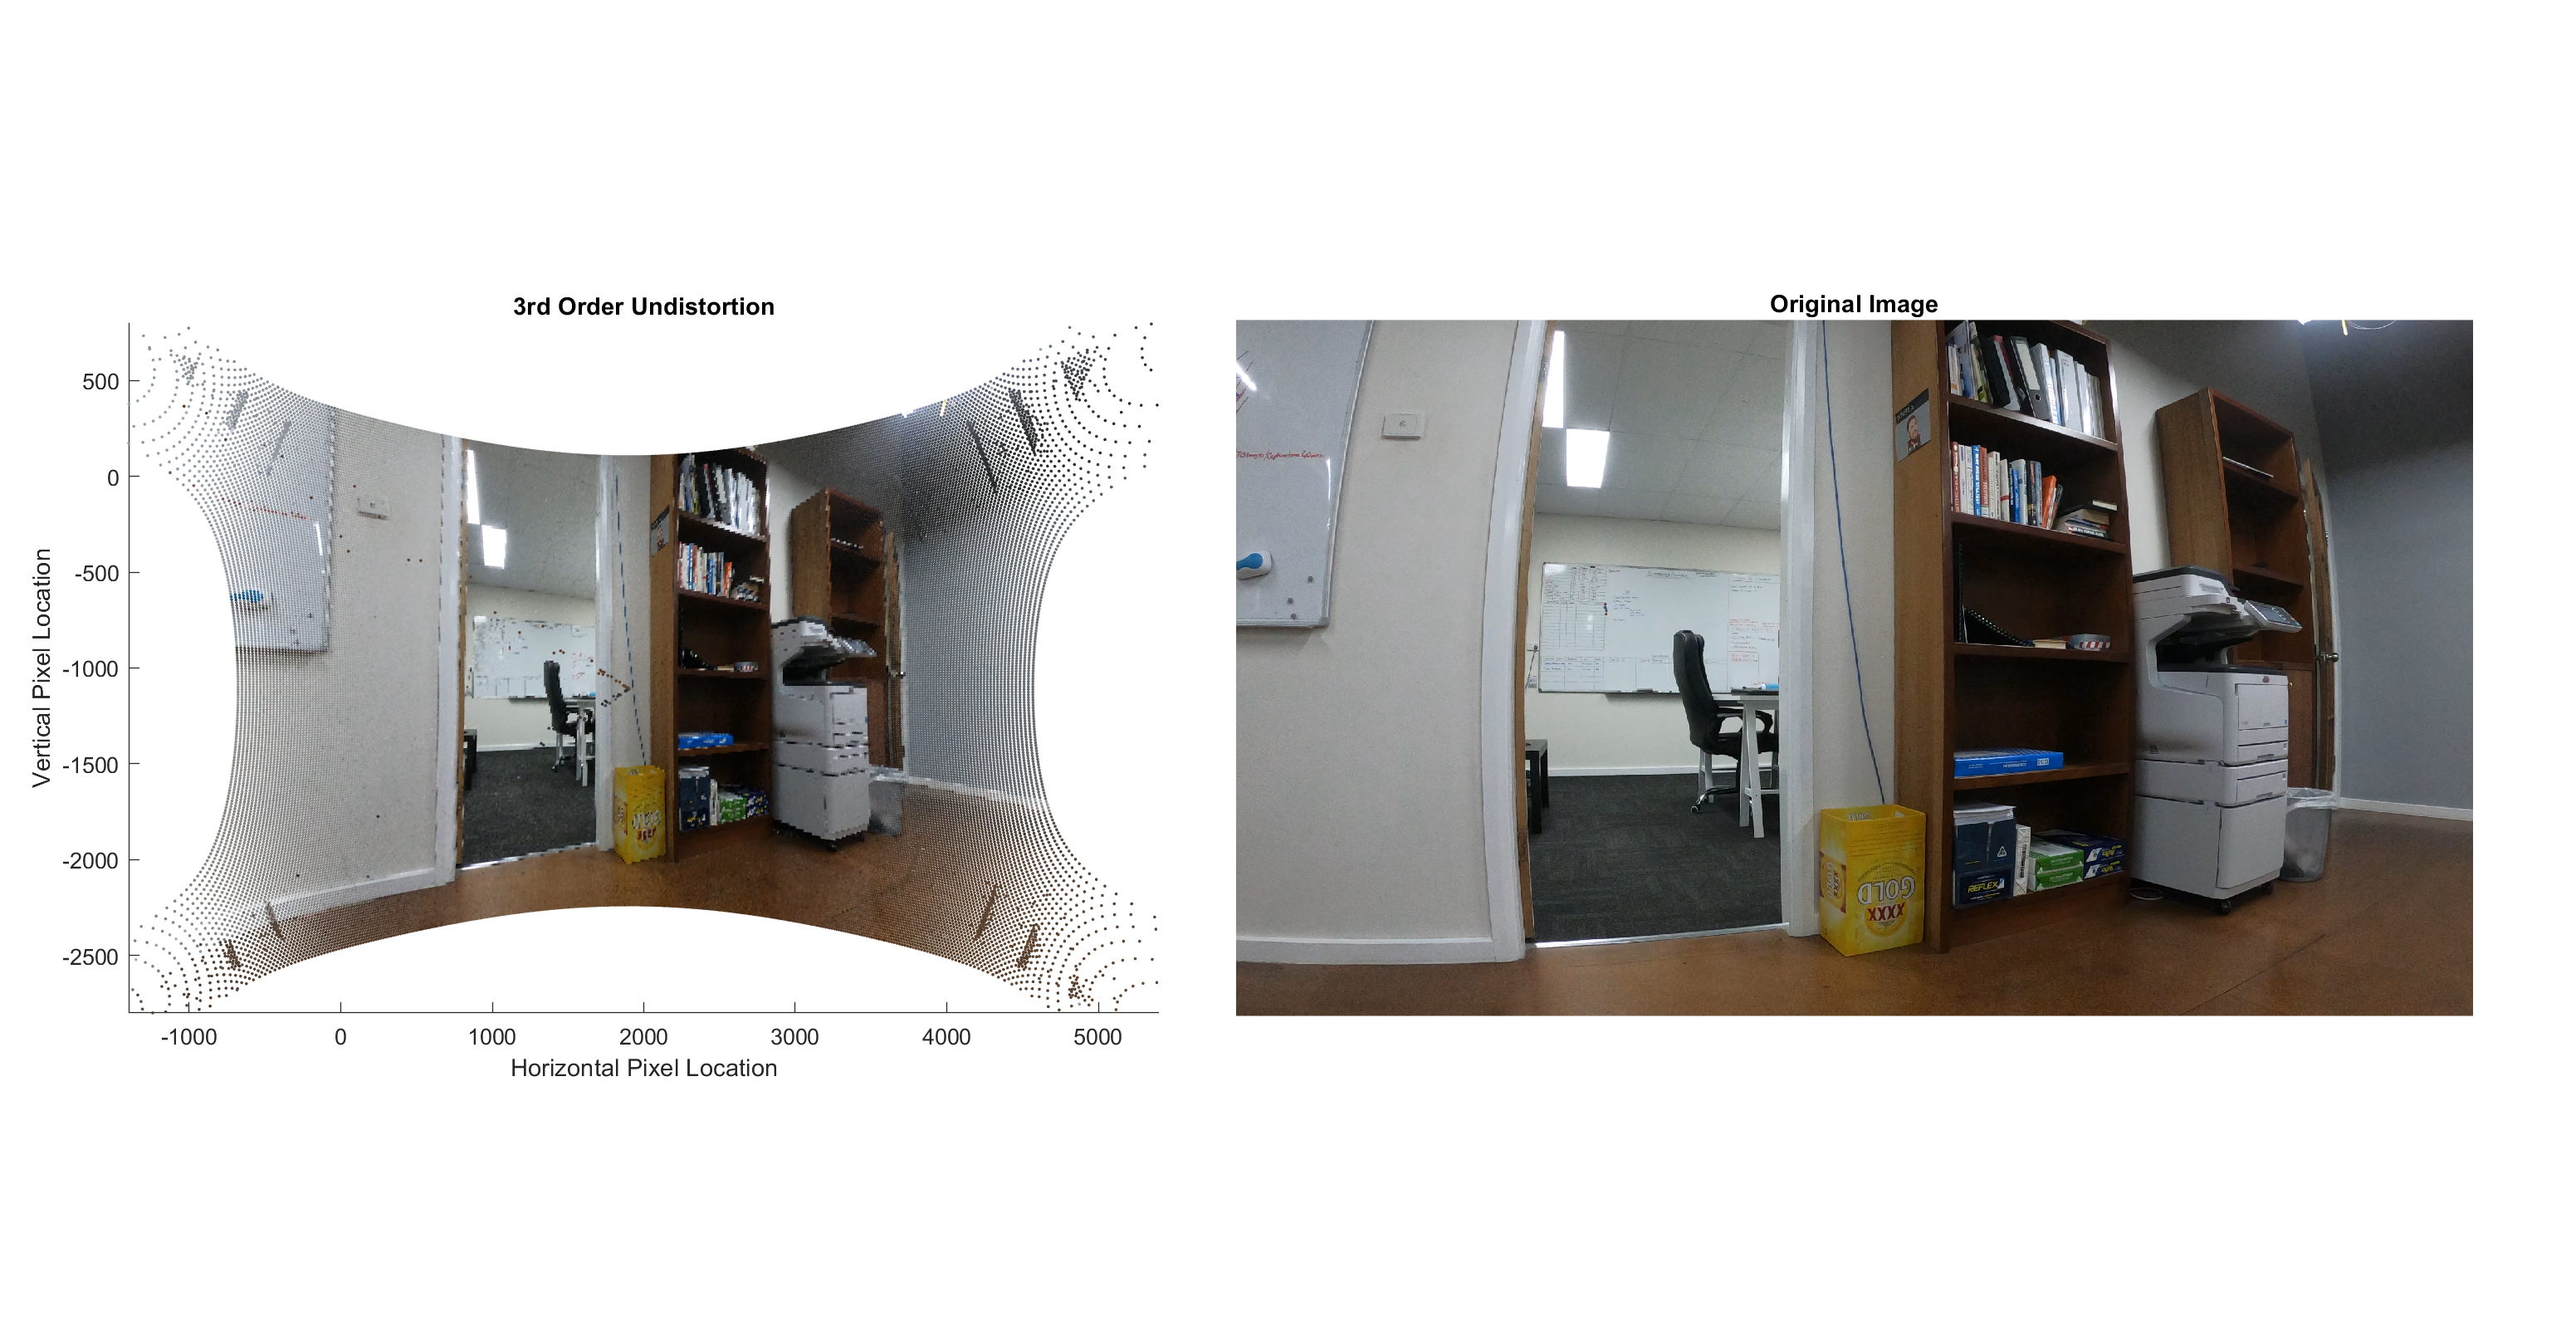
\includegraphics[width=.8\linewidth]{Figures/Matlab/3rdOrderUndistort}
        \caption{Caption}
        \label{fig:3rdOrderUndistort}
    \end{center}
\end{figure}
\begin{figure}[ht]
    \begin{center}
        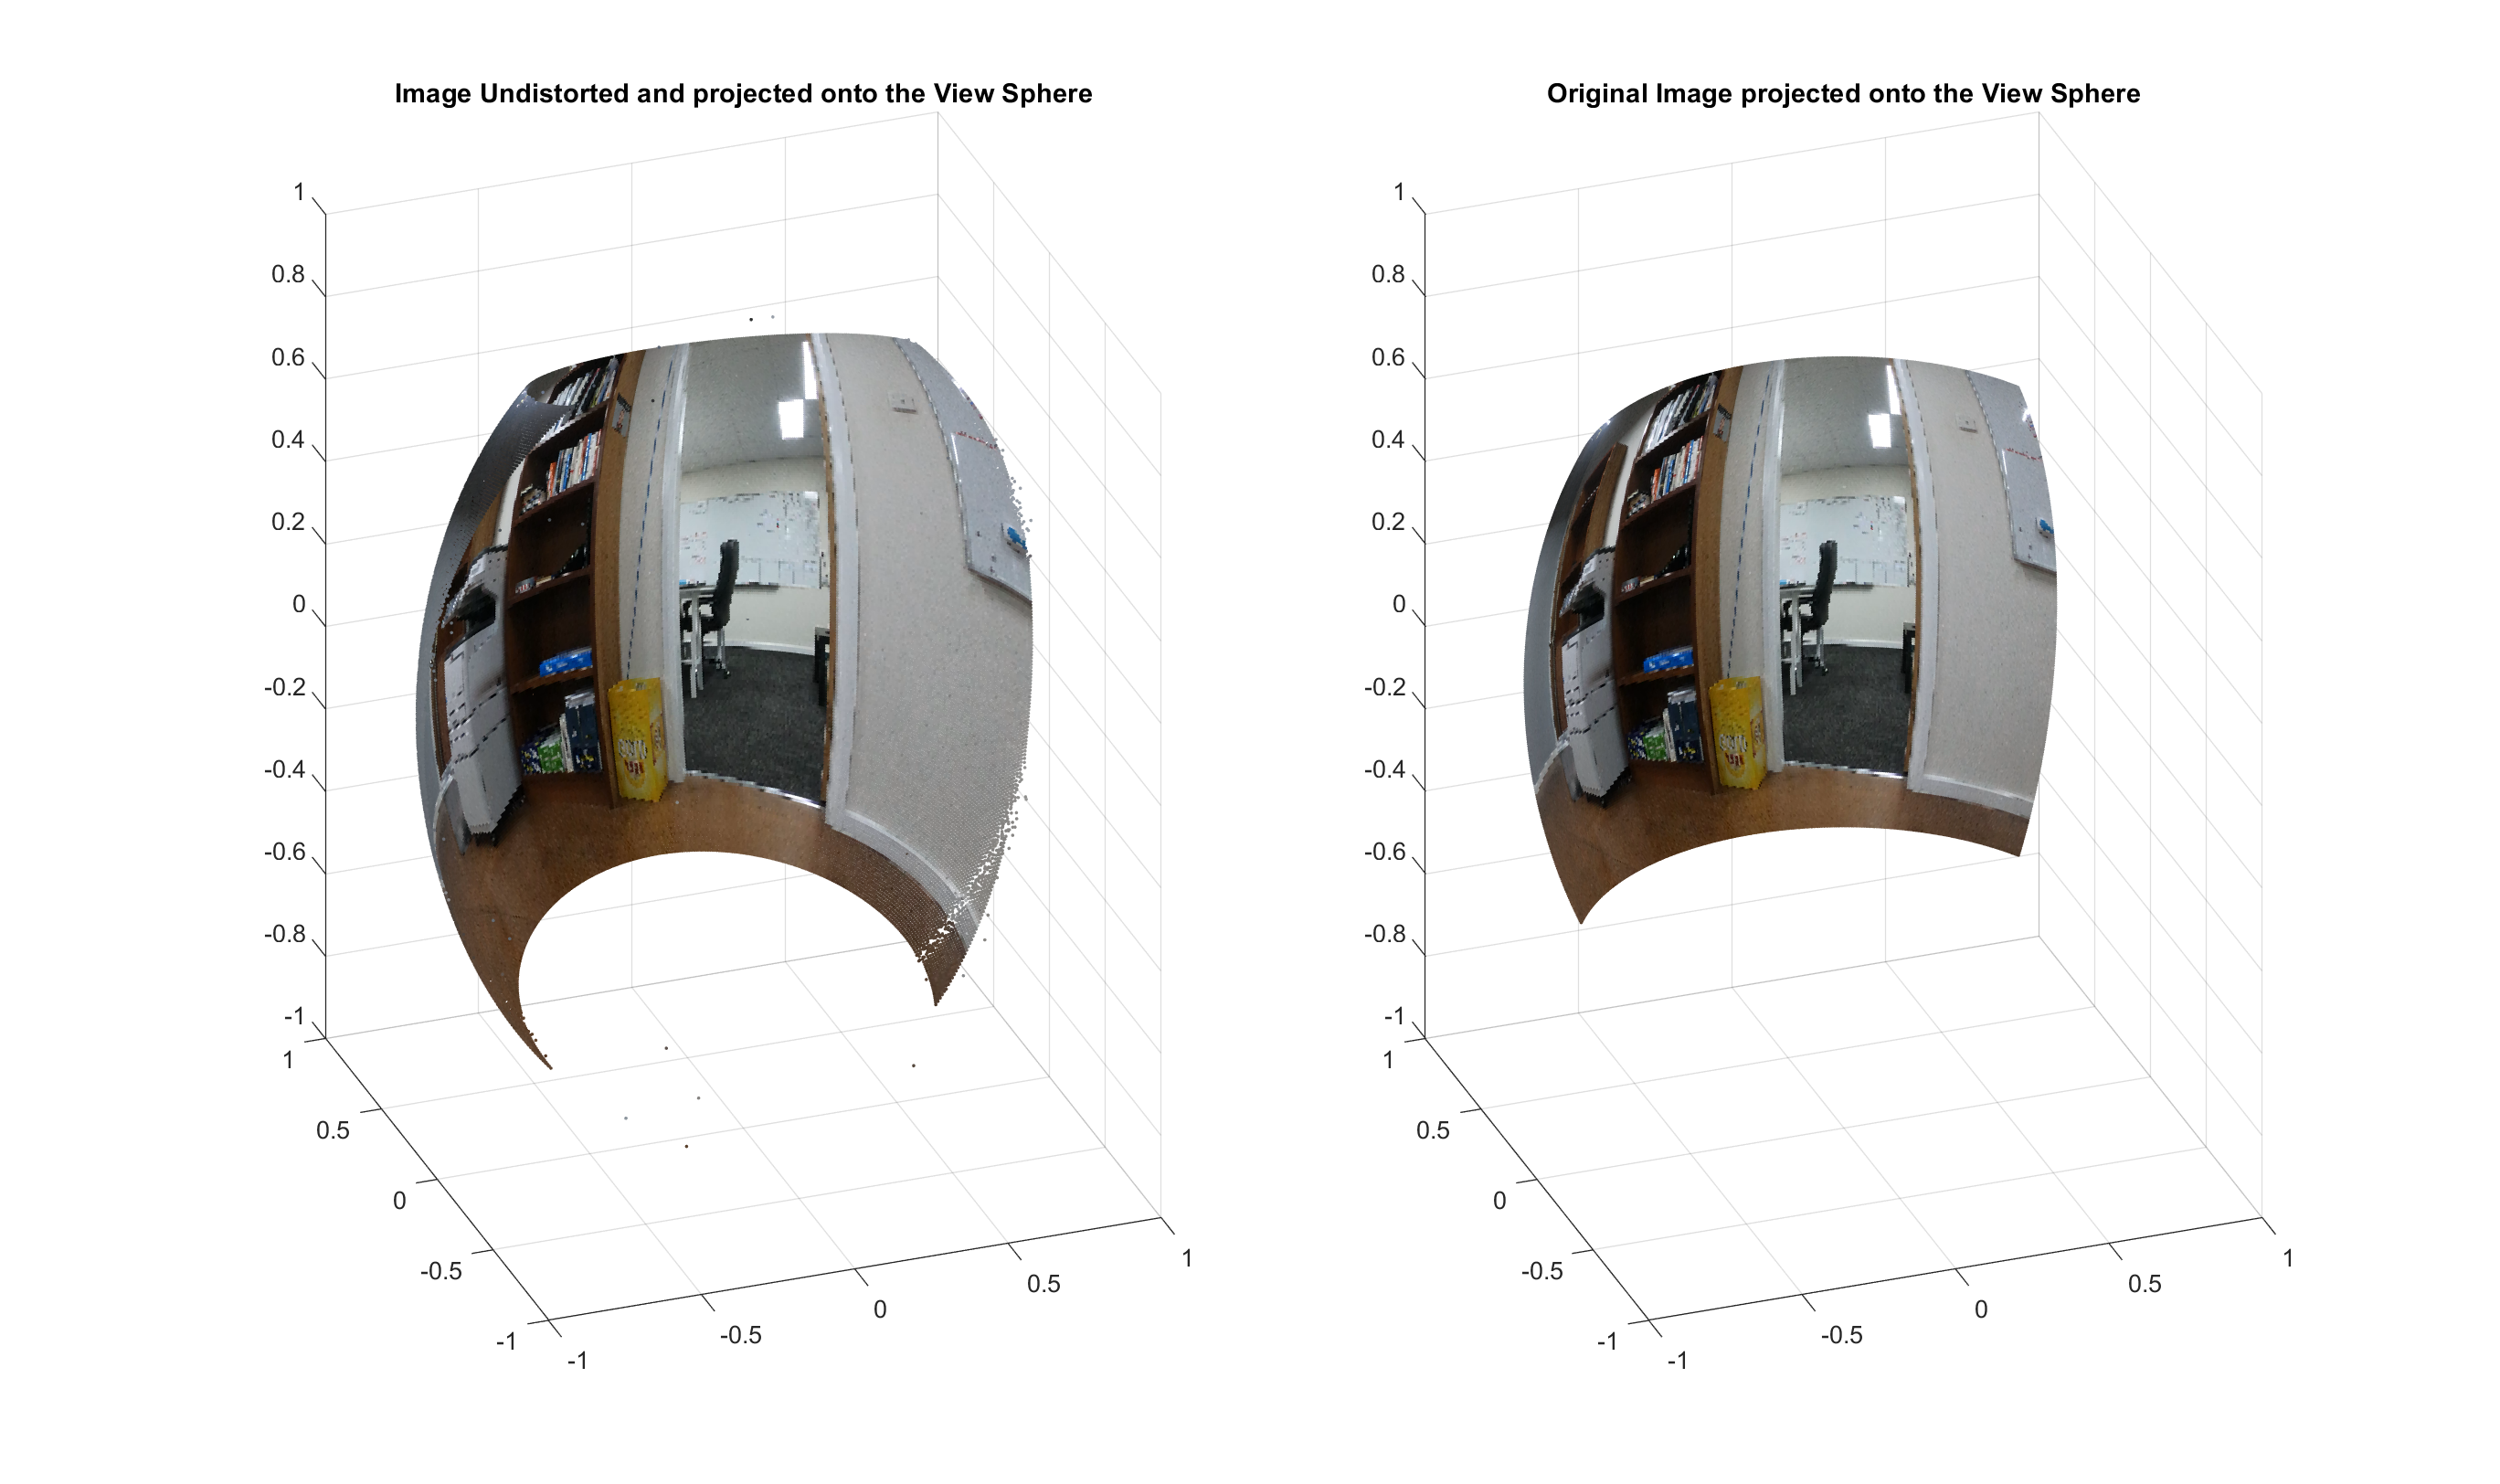
\includegraphics[width=.8\linewidth]{Figures/Matlab/Image_on_ViewSphere}
        \caption{Caption}
        \label{fig:Image_on_ViewSphere}
    \end{center}
\end{figure}
%%%%%%%%%%%%%%%%%%%%%%%%%%%%%%%
\newpage
\section{Vector Field Divergence for Object Avoidance}
\begin{figure}[ht]
    \begin{center}
        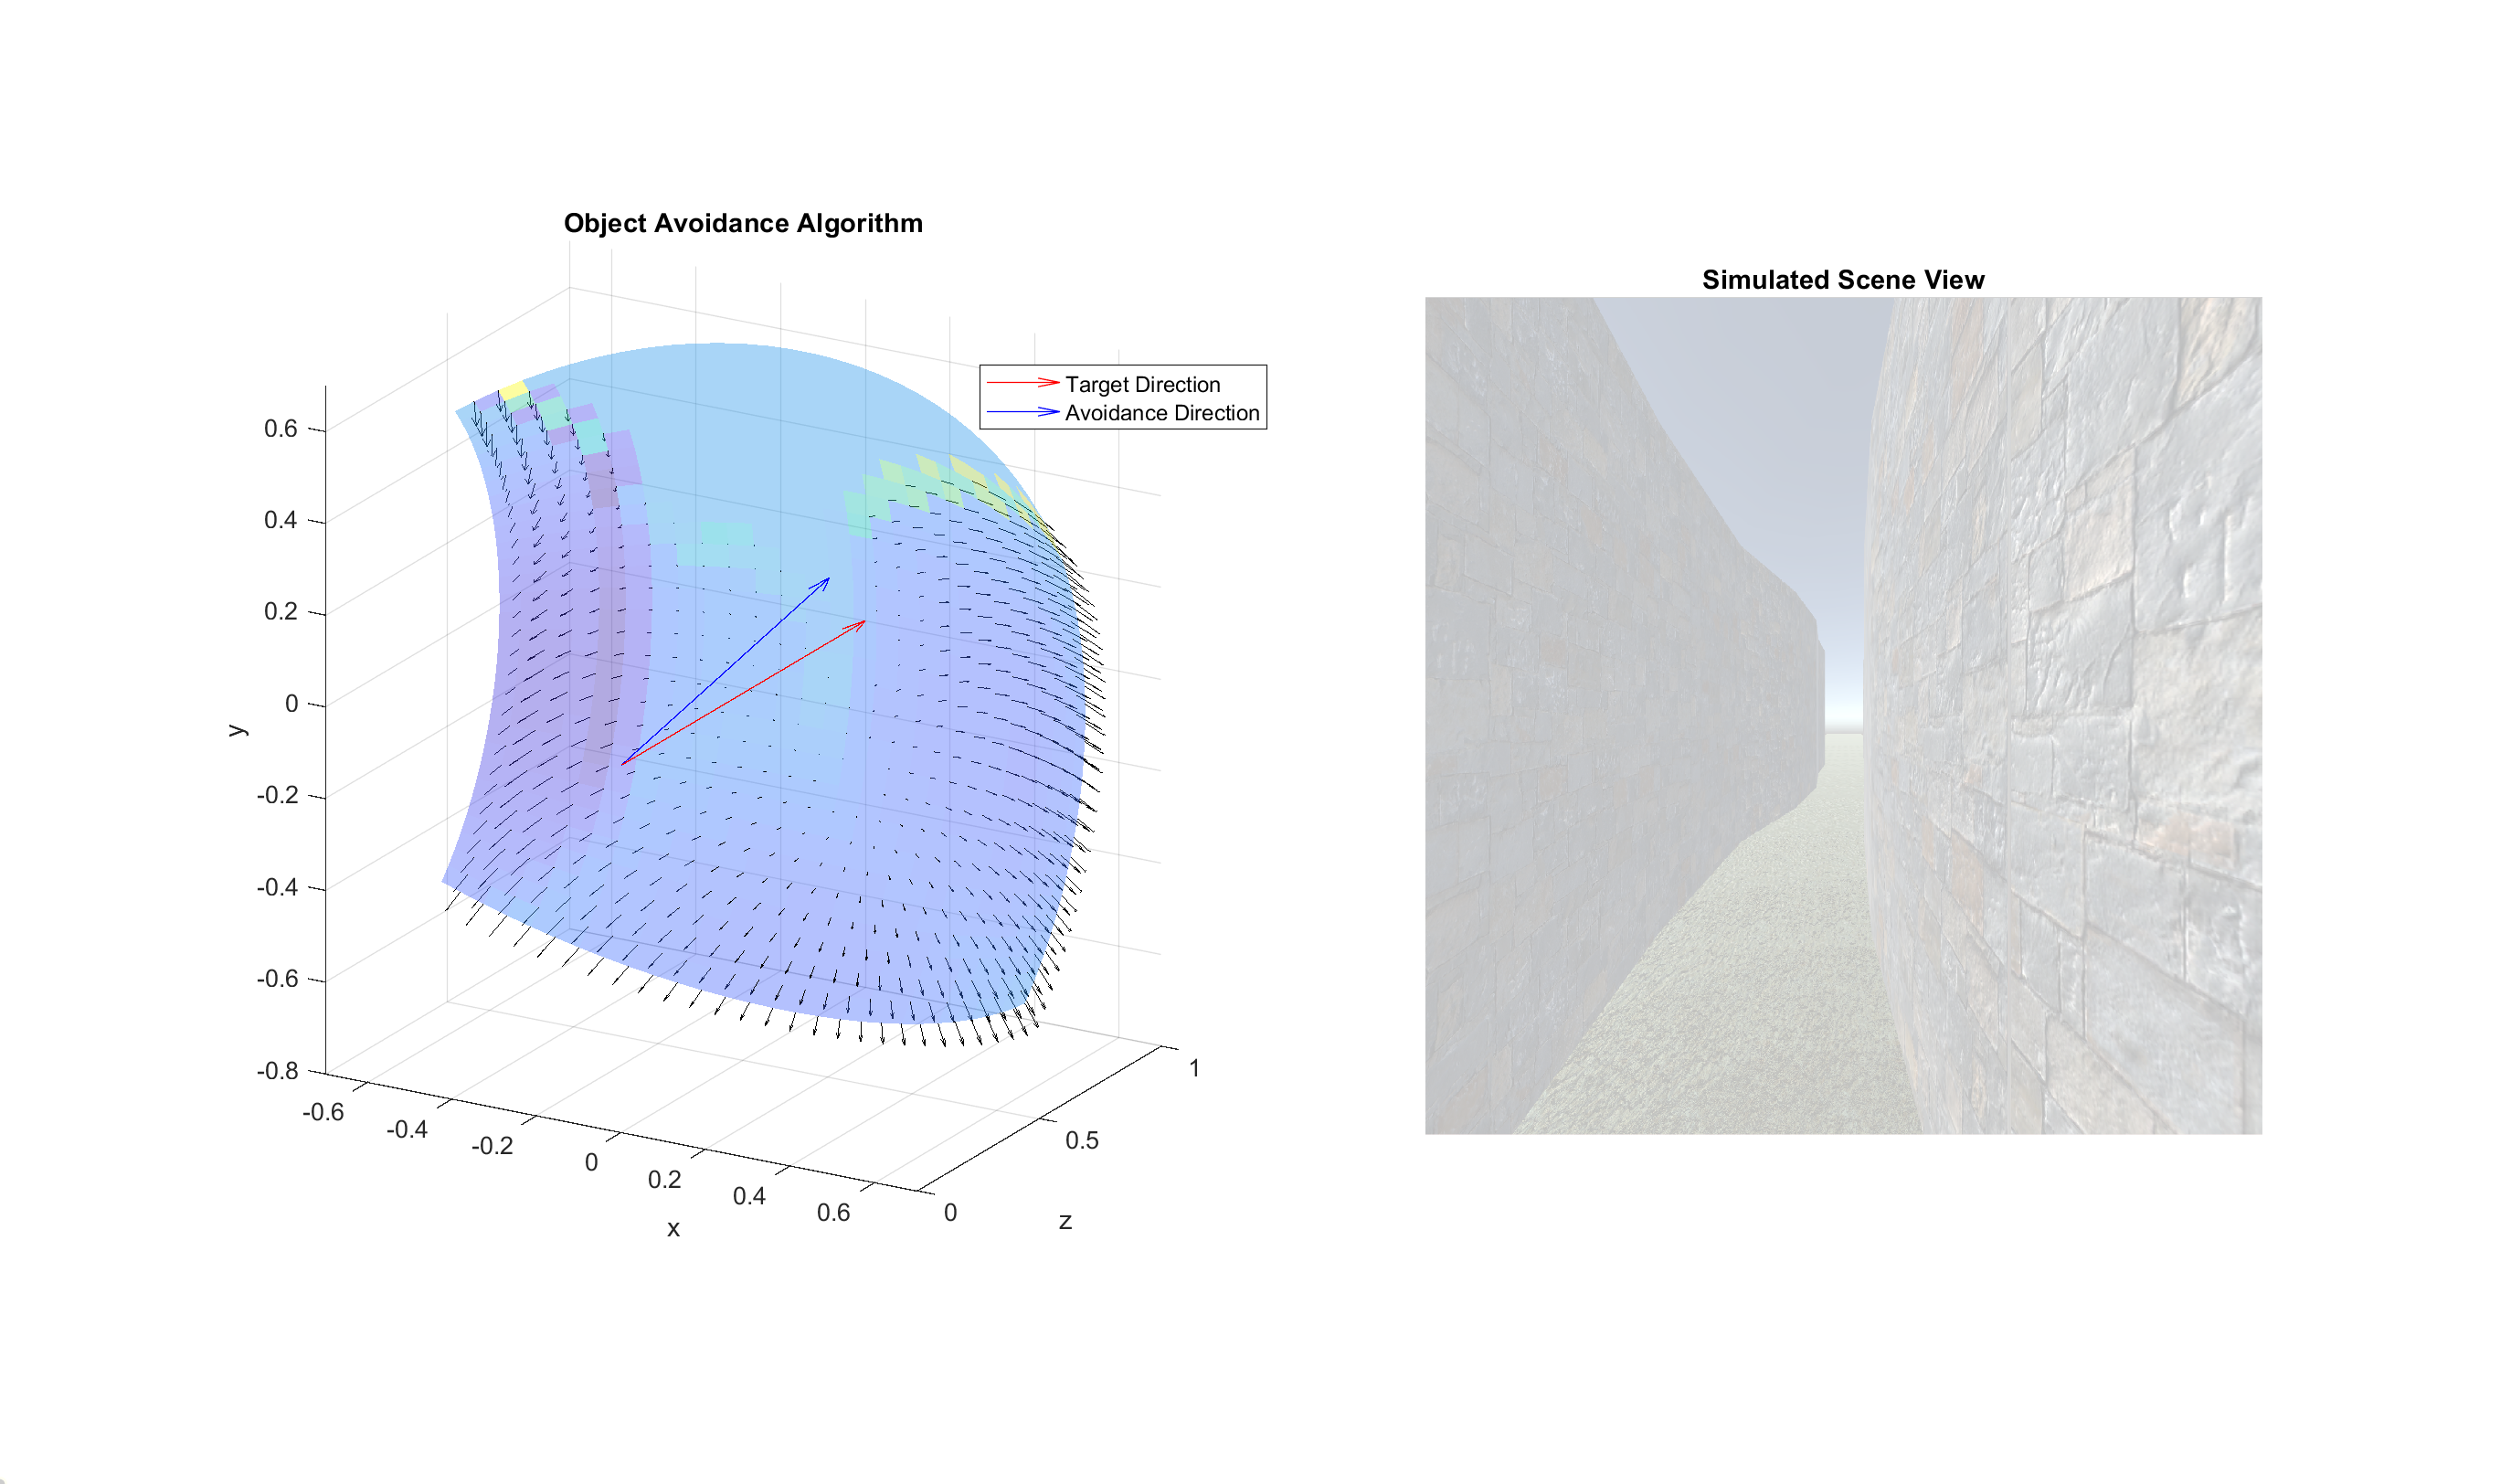
\includegraphics[width=.8\linewidth]{Figures/Matlab/Avoidance_Algorithm}
        \caption{Caption}
        \label{fig:Avoidance_Algorithm}
    \end{center}
\end{figure}

%%%%%%%%%%%%%%%%%%%%%%%%%%%%%%%
\newpage
\section{Discussion}
Environment navigation is an extremely broard topic, and this project contributes a small amout towards the obstacl avoidance 
%%%%%%%%%%%%%%%%%%%%%%%%%%%%%%%
\newpage
\section{Conclusion}\label{sec:Conclusion}
The goal of this project was to investigate the plausability of using optical flow cues as a method for avoiding obstacles in a scene. Results of the simulations show that the a cost function based on divergence of an optical flow field generates a suitable control policy, stearing the UAV in a direction away from obstacles such as walls and buildings. 

%%%%%%%%%%%%%%%%%%%%%%%%%%%%%%%
\newpage
\section{Recomendations}
For the results of this project to be implemented on a robotic platform, an optical flow algoithm would need to be run in real time. for this, an image flow algorithm that can be implemented on a descrete graphic card should be implemented such as that ceated by \cite{adarve2016filter}.


%%%%%%%%%%%%%%%%%%%%%%%%%%%%%%%
\newpage
\bibliographystyle{harvard}
\bibliography{main} % This is the .bib file where the bibliography database is stored

%%%%%%%%%%%%%%%%%%%%%%%%%%%%%%%
\appendix
\newpage
\section{Journal}\label{app:Journal}
\newpage
\section{Calibration Tool}\label{app:calibrationTool}
\begin{figure}[ht]
    \begin{center}
        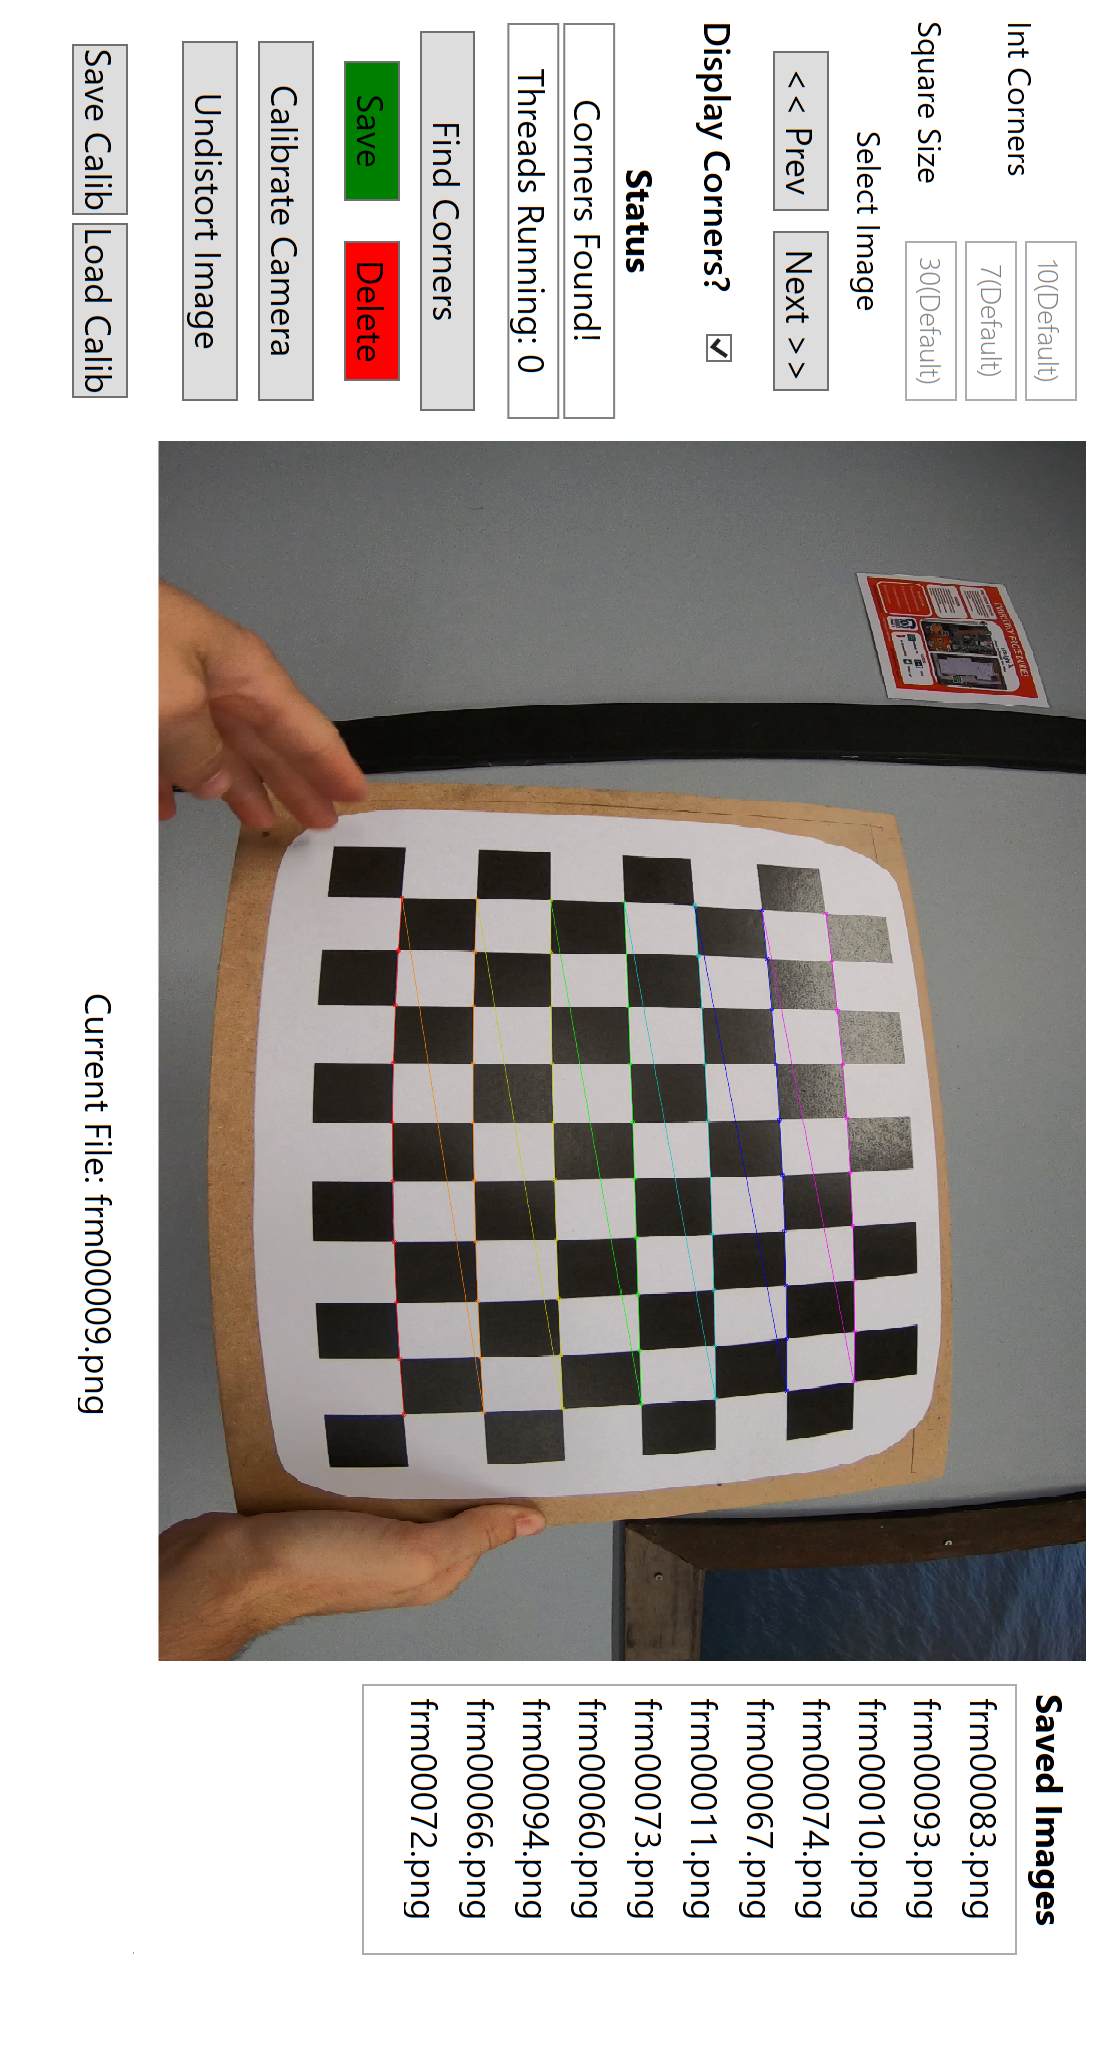
\includegraphics[width=.6\linewidth]{Figures/Calibration_Tool}
        \caption{Write something here}
        \label{fig:Calibration_Tool}
    \end{center}
\end{figure}

\end{document}